\documentclass[11pt, oneside]{article}   	% use "amsart" instead of "article" for AMSLaTeX format
\usepackage[margin = 1in]{geometry}                		% See geometry.pdf to learn the layout options. There are lots.
\geometry{letterpaper}                   		% ... or a4paper or a5paper or ... 
%\geometry{landscape}                		% Activate for rotated page geometry
%\usepackage[parfill]{parskip}    		% Activate to begin paragraphs with an empty line rather than an indent
\usepackage{graphicx}				% Use pdf, png, jpg, or eps§ with pdflatex; use eps in DVI mode
								% TeX will automatically convert eps --> pdf in pdflatex		
\usepackage{amssymb}
\usepackage{amsmath}
\usepackage[shortlabels]{enumitem}
\usepackage{float}
\usepackage{tikz-cd}
\usepackage{subcaption}
\usepackage{slashed}

\usepackage{amsthm}
\theoremstyle{definition}
\newtheorem{definition}{Definition}[section]
\newtheorem{theorem}{Theorem}[section]
\newtheorem{corollary}{Corollary}[theorem]
\newtheorem{lemma}[theorem]{Lemma}

\newcommand{\N}{\mathbb{N}}
\newcommand{\R}{\mathbb{R}}
\newcommand{\Z}{\mathbb{Z}}
\newcommand{\Q}{\mathbb{Q}}

\usepackage{simpler-wick}
\usepackage[compat=1.0.0]{tikz-feynman}   %note you need to compile this in LuaLaTeX for diagrams to render correctly

% make arrow superscripts
\DeclareFontFamily{OMS}{oasy}{\skewchar\font48 }
\DeclareFontShape{OMS}{oasy}{m}{n}{%
         <-5.5> oasy5     <5.5-6.5> oasy6
      <6.5-7.5> oasy7     <7.5-8.5> oasy8
      <8.5-9.5> oasy9     <9.5->  oasy10
      }{}
\DeclareFontShape{OMS}{oasy}{b}{n}{%
       <-6> oabsy5
      <6-8> oabsy7
      <8->  oabsy10
      }{}
\DeclareSymbolFont{oasy}{OMS}{oasy}{m}{n}
\SetSymbolFont{oasy}{bold}{OMS}{oasy}{b}{n}

\DeclareMathSymbol{\smallleftarrow}     {\mathrel}{oasy}{"20}
\DeclareMathSymbol{\smallrightarrow}    {\mathrel}{oasy}{"21}
\DeclareMathSymbol{\smallleftrightarrow}{\mathrel}{oasy}{"24}
%\newcommand{\cev}[1]{\reflectbox{\ensuremath{\vec{\reflectbox{\ensuremath{#1}}}}}}
\newcommand{\vecc}[1]{\overset{\scriptscriptstyle\smallrightarrow}{#1}}
\newcommand{\cev}[1]{\overset{\scriptscriptstyle\smallleftarrow}{#1}}
\newcommand{\cevvec}[1]{\overset{\scriptscriptstyle\smallleftrightarrow}{#1}}

\newcommand{\dbar}{d\hspace*{-0.08em}\bar{}\hspace*{0.1em}}

\usepackage{tcolorbox}
\tcbuselibrary{theorems}
\newtcolorbox{answerbox}{sharp corners=all, colframe=black, colback=black!5!white, boxrule=1.5pt, halign=flush center, width = 1\textwidth, valign=center}
\newenvironment{answer}{\begin{center}\begin{answerbox}}{\end{answerbox}\end{center}}

\title{Instantons and Solitons}
\author{Patrick Oare}
\date{}							% Activate to display a given date or no date

\begin{document}
\maketitle

\section{Overview}

Instantons and solitons are solutions which arise to the classical field equations which are intimately tied to the topological properties of our 
fields. Instantons are classical solutions to the field equations which occur over time as we study the limits of our theory with $t\rightarrow\pm 
\infty$, and solitons are time-independent solutions. These are inherently non-perturbative phenomena, and they will not show up at 
any order in perturbation theory. 

We will study both of these in a semi-classical limits. We will be interested in solutions to the classical equations of motion for our theory; 
solitons and instantons can be treated by approximating the path-integral with the steepest descent method, where the stationary points 
of the action (classical solutions) with $\delta S|_{\phi_0} = 0$ are the main contributors to matrix elements. We will do this rigorously 
in the next section, but for now we may note that (in Euclidean time) this approximation takes the form:
\begin{equation}
	\int D\phi e^{-S[\phi] / \hbar}\sim C e^{-S[\phi_0] / \hbar} (1 + \mathcal O(\hbar))
\end{equation}
where $\phi_0$ is a classical solution to the field equations that makes the action stationary. Instanton and soliton solutions will have the 
property that if we examine $S[\phi_0]$, we will see that $S[\phi_0]\sim 1 / \lambda$, or some power of this, where $\lambda$ is the coupling 
constant. Since perturbation theory expands the action in powers of $\lambda$, we can see explicitly that \textbf{such a solution will have 
non-perturbative effects because $e^{-\frac{1}{\lambda}}$ is non-analytic} and cannot be expanded in a power series. 

% Do the 1D example
Instantons and solitons are topological objects at their core. They essentially measure the ``twisting" of a field on the boundary of spacetime 
into the set of vevs that the field can take on, and as such are often connected to spontaneous symmetry breaking. As an example, consider 
the double well potential in a (1 + 1)d field theory:
\begin{equation}
	V(\phi) = \frac{1}{8}\lambda (\phi^2 - v^2)^2
\end{equation}

This potential is plotted in Figure~\ref{subfig:double_well}. This theory has two vacua, $\pm v$, and the original symmetry group of 
$\mathbb Z / 2\mathbb Z$ is spontaneously broken. A classical field configuration which minimizes the energy of the theory must 
therefore approach either $v$ or $-v$ asymptotically as $x\rightarrow\infty$. These can be topologically trivial and stay in the 
same vacuum as $x\rightarrow\pm \infty$, or they can be interesting and interpolate between the two vacua. A nontrivial solution 
which begins in the $-v$ vacuum and ends in the $+v$ vacuum is depicted in Figure~\ref{subfig:double_well_soliton}. 

This solution is interesting because we can look at its energy: it is called a \textbf{soliton}. Recall the energy scales in our problem: 
the $\phi$ boson gains a mass through spontaneous symmetry breaking of:
\begin{equation}
	m^2 = \lambda v^2
\end{equation}
The field configuration in Figure~\ref{subfig:double_well_soliton} also has some inherent energy because of the transition it undergoes between 
the two vacua. Its energy can be evaluated classically as:
\begin{align}
	E &= \int_\mathbb{R}dx\left[\frac{1}{2}(\phi')^2 + V(\phi)\right] = \frac{1}{2}\int_\mathbb{R}dx \left(\phi' - \sqrt{2V(\phi)}\right)^2 + \int_{-v}^v d\phi \sqrt{2V(\phi)} \nonumber \\
	   &= \frac{1}{2}\int_\mathbb{R}dx \left(\phi' - \sqrt{2V(\phi)}\right)^2 + \left(\frac{2m^2}{3\lambda}\right) m
\end{align}
where $\dot\phi = 0$ because this is a time-independent solution. The first term is positive definite, and the second term is a result of the field 
changing vacuums. We see that for our field configuration to satisfy $\phi(\pm x) = \pm v$, it must have an energy of at least
\begin{equation}
	M = \left(\frac{2m^2}{3\lambda}\right) m.
\end{equation}
This is called the mass of the soliton. In the weak coupling limit with $\lambda << m^2$, the soliton mass is $M >> m$ and introduces a heavy scale into the 
problem. Furthermore, it is topologically protected: it would require an \textit{infinite amount of energy} to remove the kink from the field configuration, 
as we would have to put in the energy to flatten out the curve in Figure~\ref{subfig:double_well_soliton} at an uncountable number of points. Putting a finite 
amount of work into trying to change the field configuration to a trivial one would only serve to move the kink along the real line, and wouldn't remove this 
massive excitation from the theory. We can change frames and boost the kink, and it acts like a particle; upon a Lorentz boost with parameter $\gamma$, 
the soliton's energy will become $E = \gamma M$, and so we can treat this field configuration as a particle of mass $M$ which can be boosted and move around 
dynamically. 

\begin{figure}[H]
	\centering
	\begin{subfigure}[t]{.38\textwidth}
		\centering
		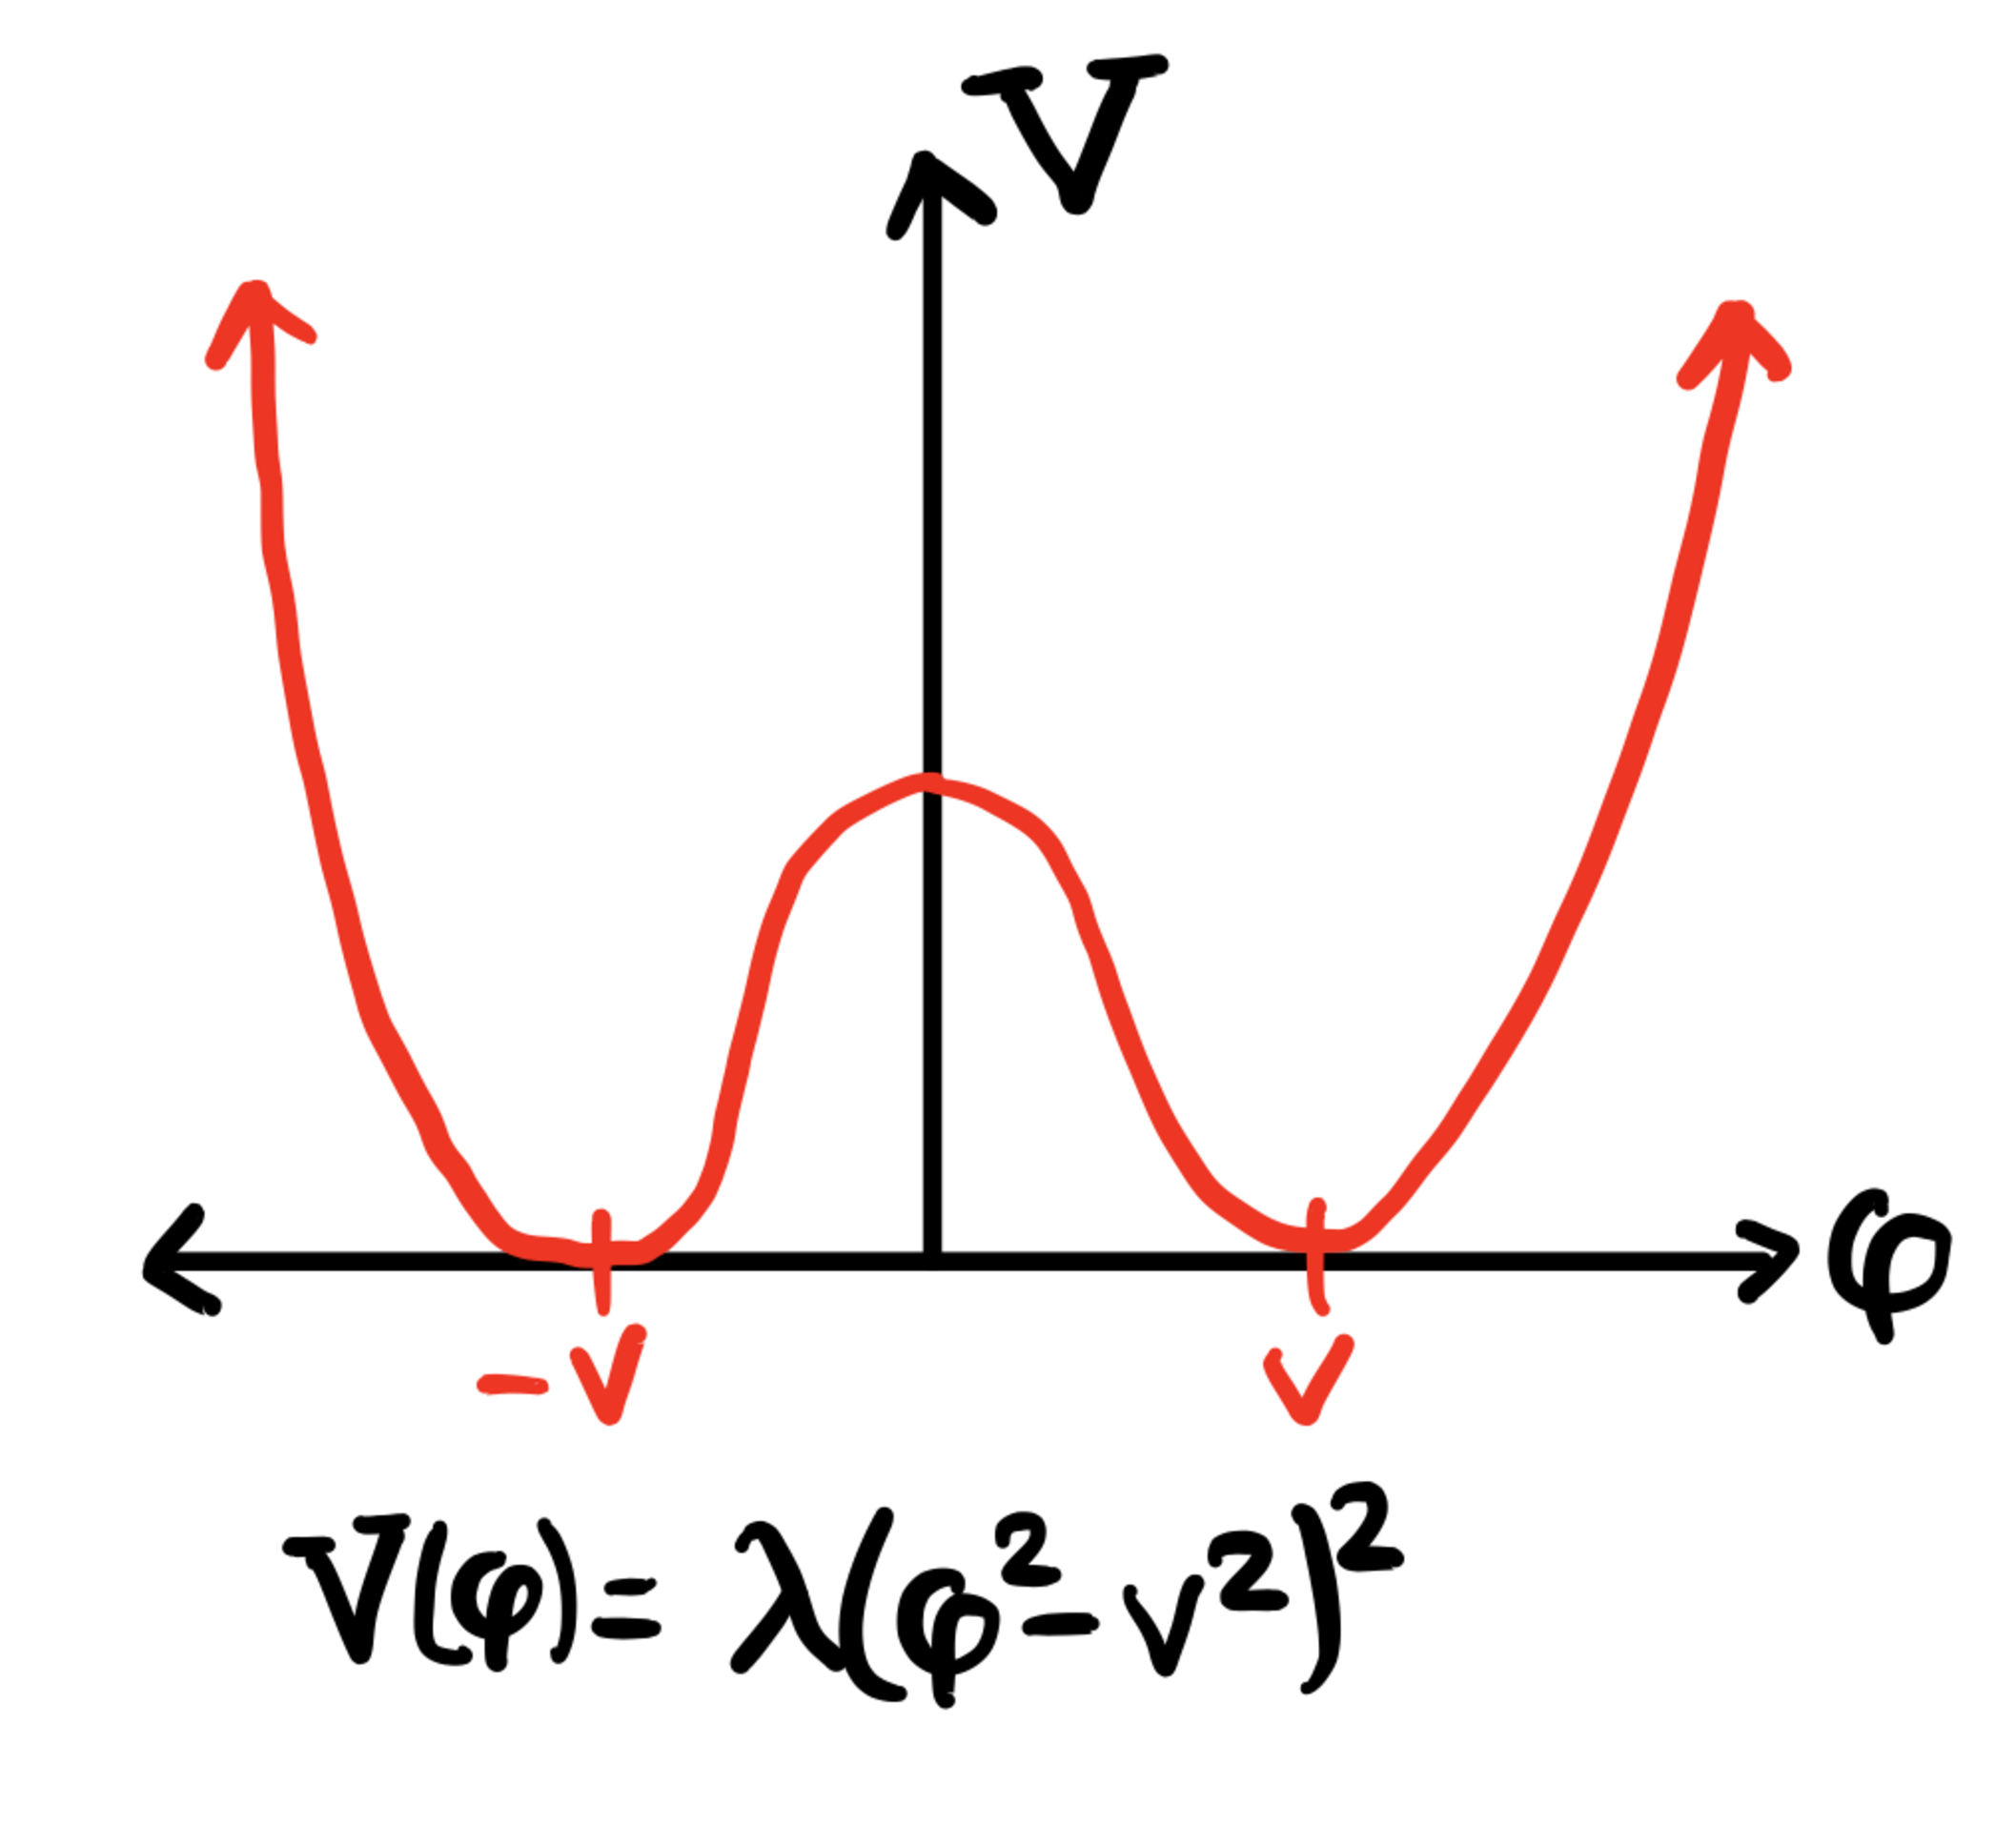
\includegraphics[width = .8\textwidth]{double_well}
		\caption{Double well potential.}~
		\label{subfig:double_well}
	\end{subfigure}
	~
	\begin{subfigure}[t]{.38\textwidth}
		\centering
		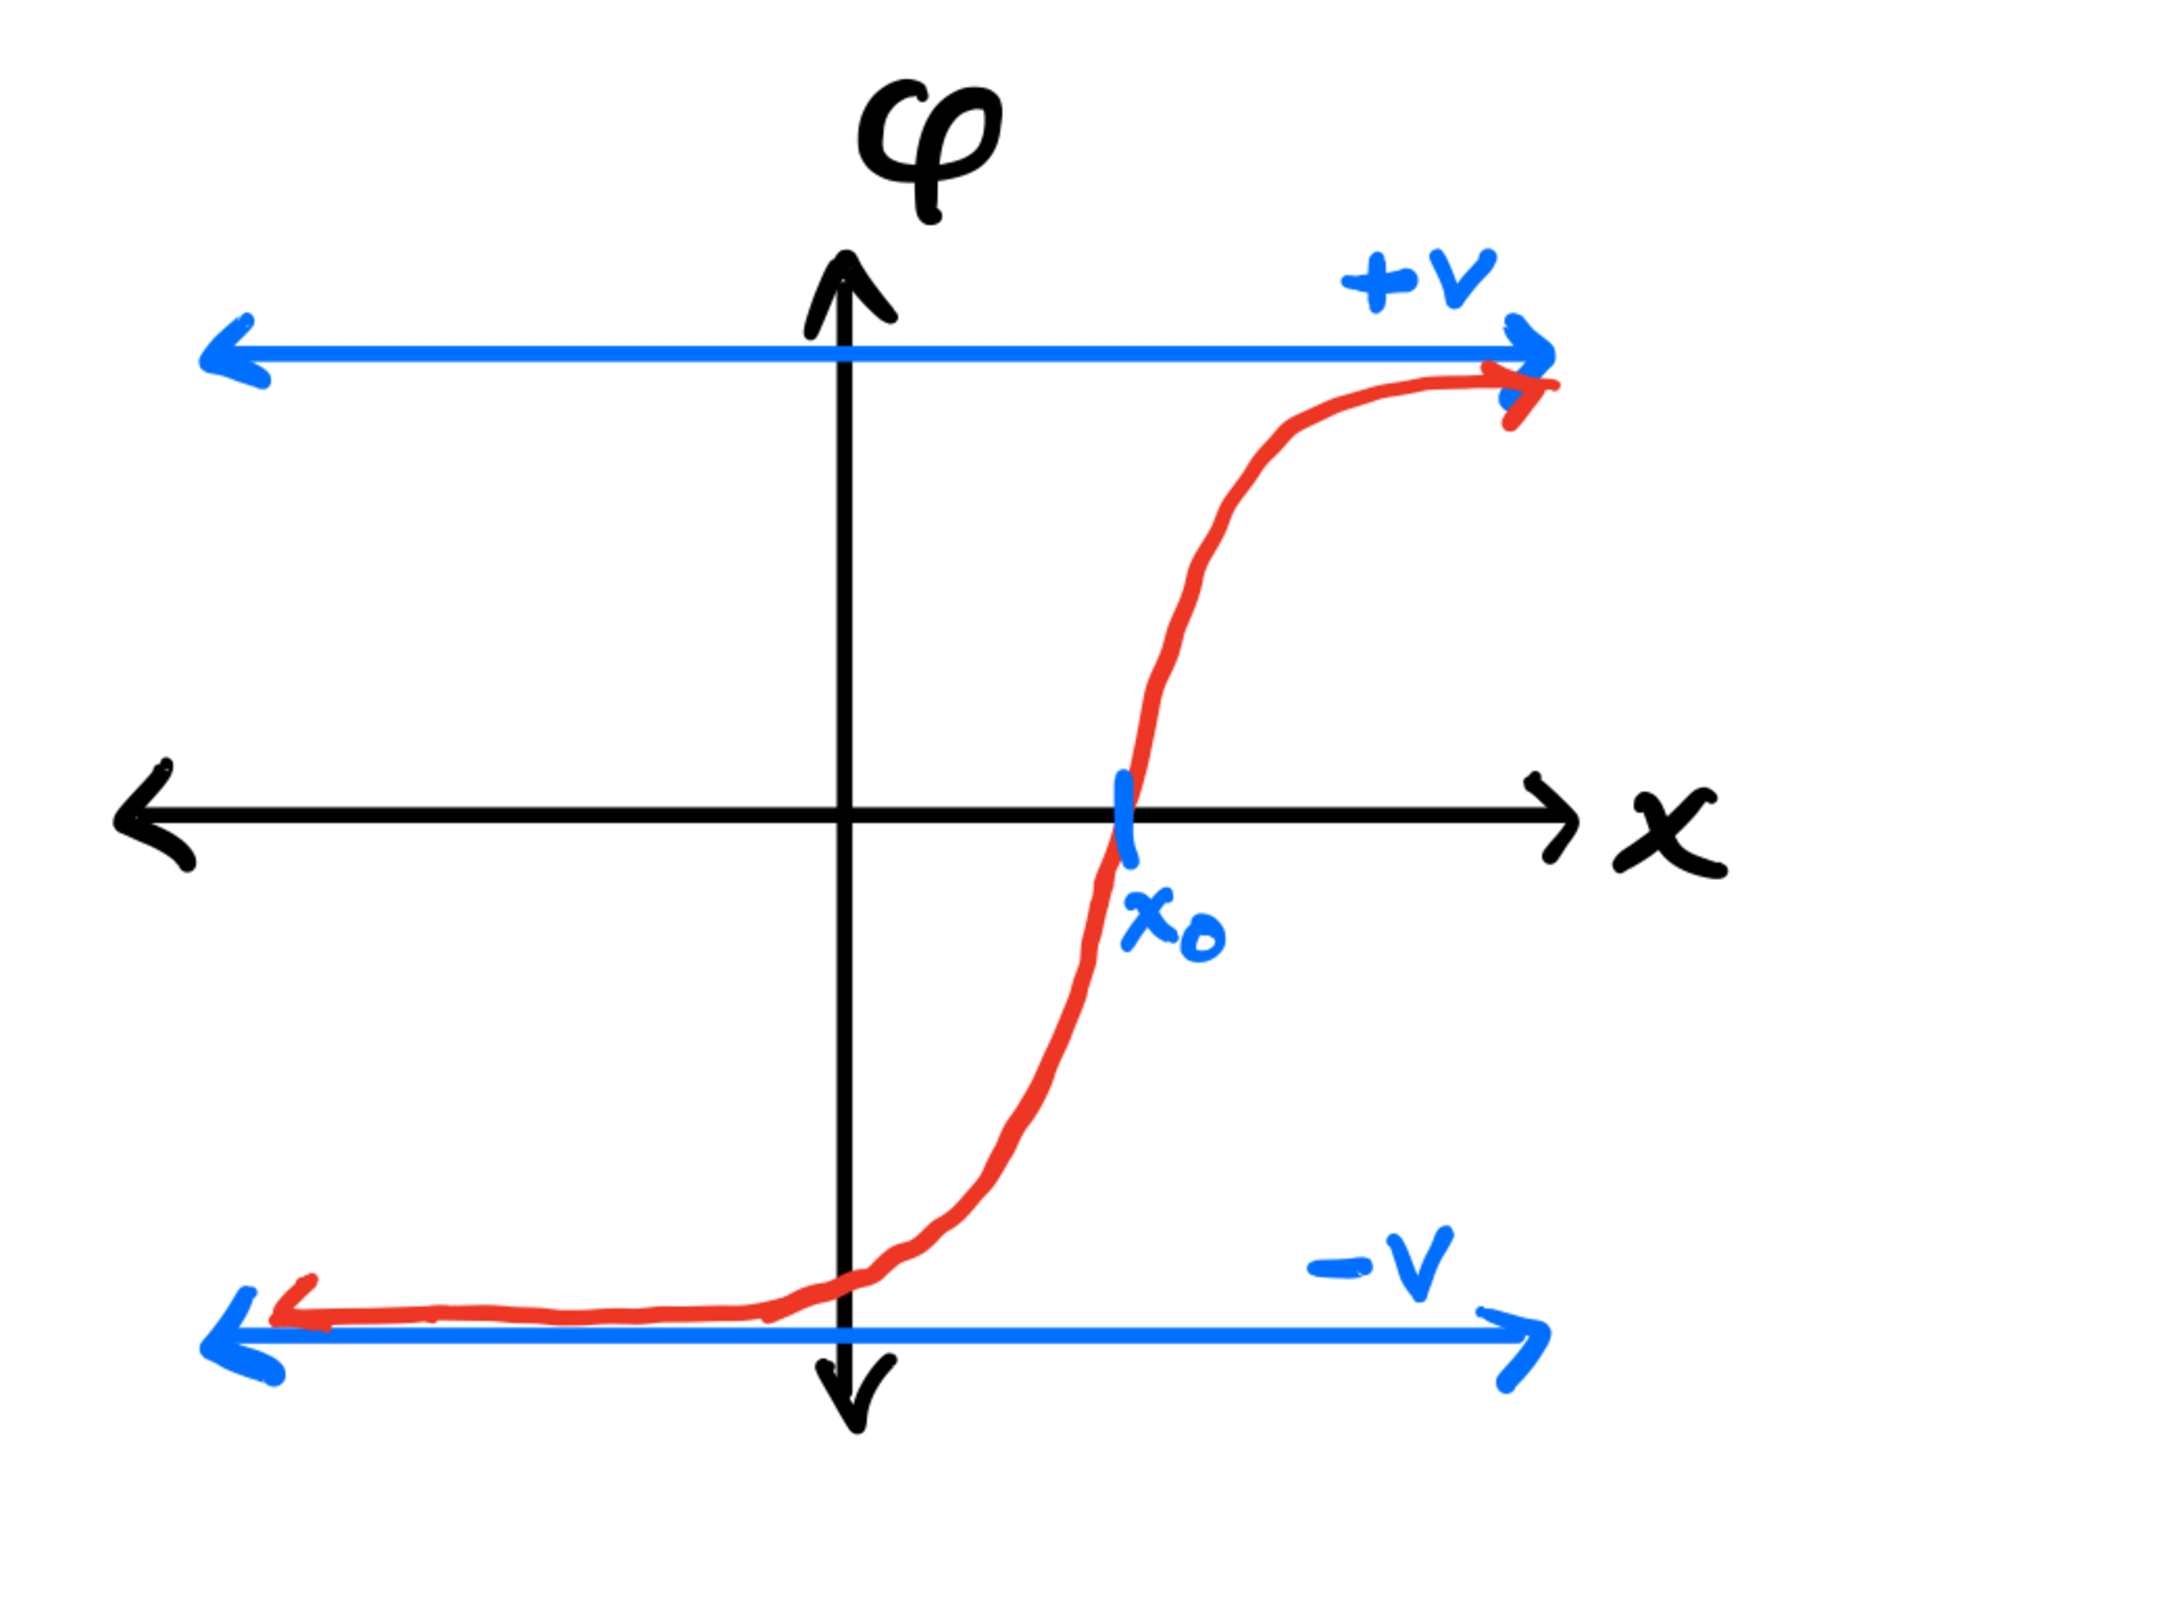
\includegraphics[width = .8\textwidth]{soliton_1d}
		\caption{Soliton solution to classical EoM with $\phi(x\rightarrow\pm\infty) = \pm v$.}~
		\label{subfig:double_well_soliton}
	\end{subfigure}
\end{figure}

The major theme that we will see in these notes is that we can classify vacuum field configurations via maps:
\begin{equation}
	\left\{\textnormal{Boundary of spacetime}\right\}\rightarrow \left\{\textnormal{Vacuum manifold}\right\}
\end{equation}
In this (1 + 1)d soliton solution, we had to map the two points on the boundary of spacetime to one of two vacuum values, $\pm v$, and 
the choices of where to map each one are topologically distinct; they cannot be deformed into one another with a finite amount of energy. 
\textit{Topologically equivalent field configurations will end up living in the same homotopy classes, and we will see that we can classify these 
classical field configurations via homotopy groups}. For now, though, we will dive into another toy model: that of tunneling in quantum 
mechanics. We will use the method of steepest descent to study tunneling quantitatively, because many of the features that are seen 
in this simple model can be ported over to QCD and more complicated field configurations relatively easily. 

\begin{answer}
	\begin{center}
		\textbf{Interlude 1: Homotopy groups}
	\end{center}
	\begin{flushleft} \setlength{\parindent}{2em}
	Homotopy is a topological property of maps which tells us about deformation. Given two maps between topological spaces $f, g: X\rightarrow Y$, 
	a \textbf{homotopy} between $f$ and $g$ is a map $h : X\times [0, 1]\rightarrow Y$ such that:
	\begin{align}
		h(x, 0) = f(x) && h(x, 1) = g(x)
	\end{align}
	for each $x\in X$. This means that $h(x, t)$ \textit{smoothly interpolates} between $f(x)$ at time $t = 0$ and $g(x)$ at time $t = 1$. One can think of 
	$h$ as a smooth deformation of $f$ into $g$. The existence of a homotopy between two maps can us a great deal about the topology of the 
	underlying space. Suppose we have two curves $\gamma_1, \gamma_2 : [a, b]\rightarrow Y$. If there is a homotopy between $\gamma_1$ and 
	$\gamma_2$ which fixes the endpoints of each curve , this tells us there are no ``holes" in the space between $\gamma_1$ and $\gamma_2$. For 
	a concrete example, check out Figures~\ref{subfig:homotopy1} and~\ref{subfig:homotopy2}. When a point between the curves is removed, they can 
	no longer be deformed continuously into one another.
	\end{flushleft}
	\begin{figure}[H]
	\centering
	\begin{subfigure}[t]{.4\textwidth}
		\centering
		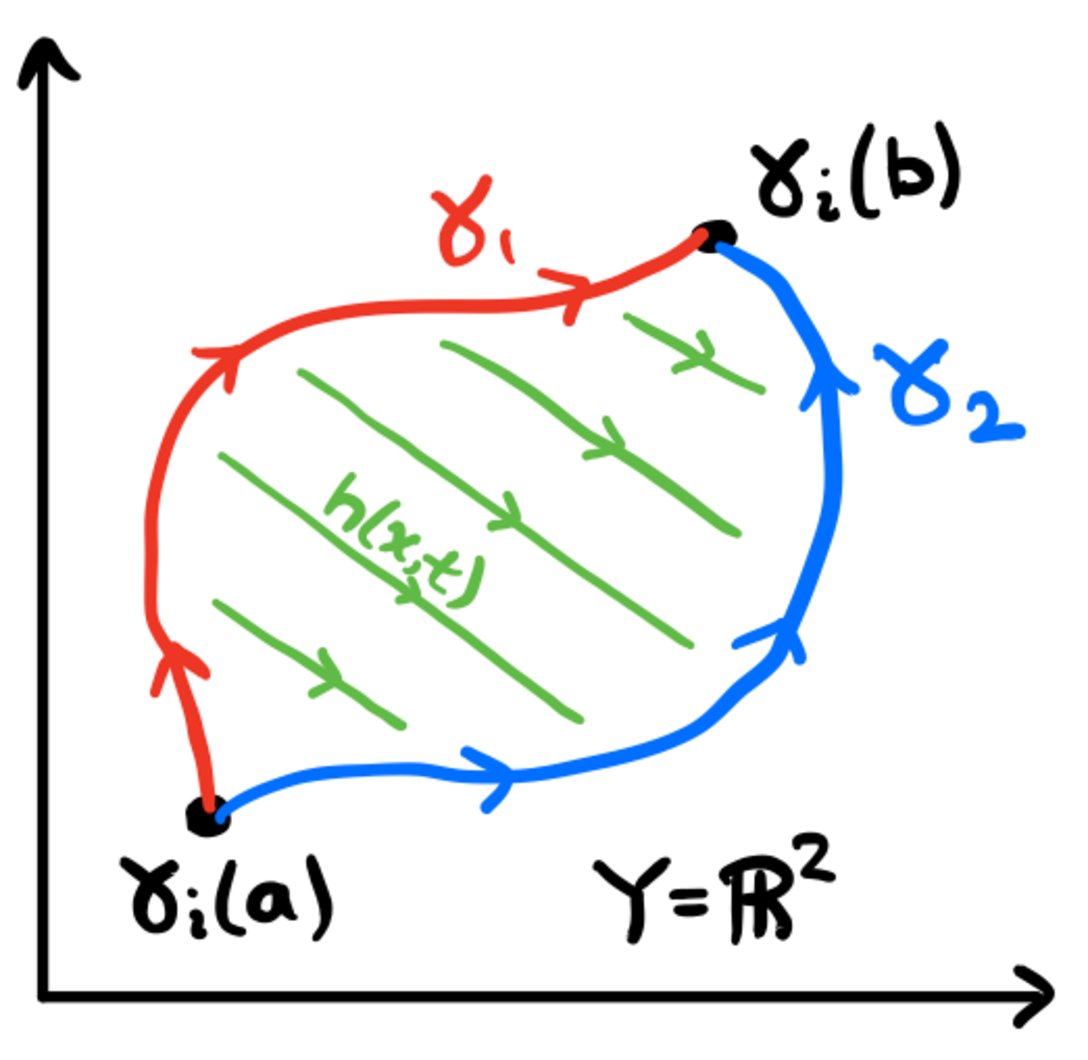
\includegraphics[width = .8\textwidth]{homotopy_1}
		\caption{A homotopy in $Y = \mathbb R^2$ from $\gamma_1$ into $\gamma_2$..}~
		\label{subfig:homotopy1}
	\end{subfigure}
	~
	\begin{subfigure}[t]{.4\textwidth}
		\centering
		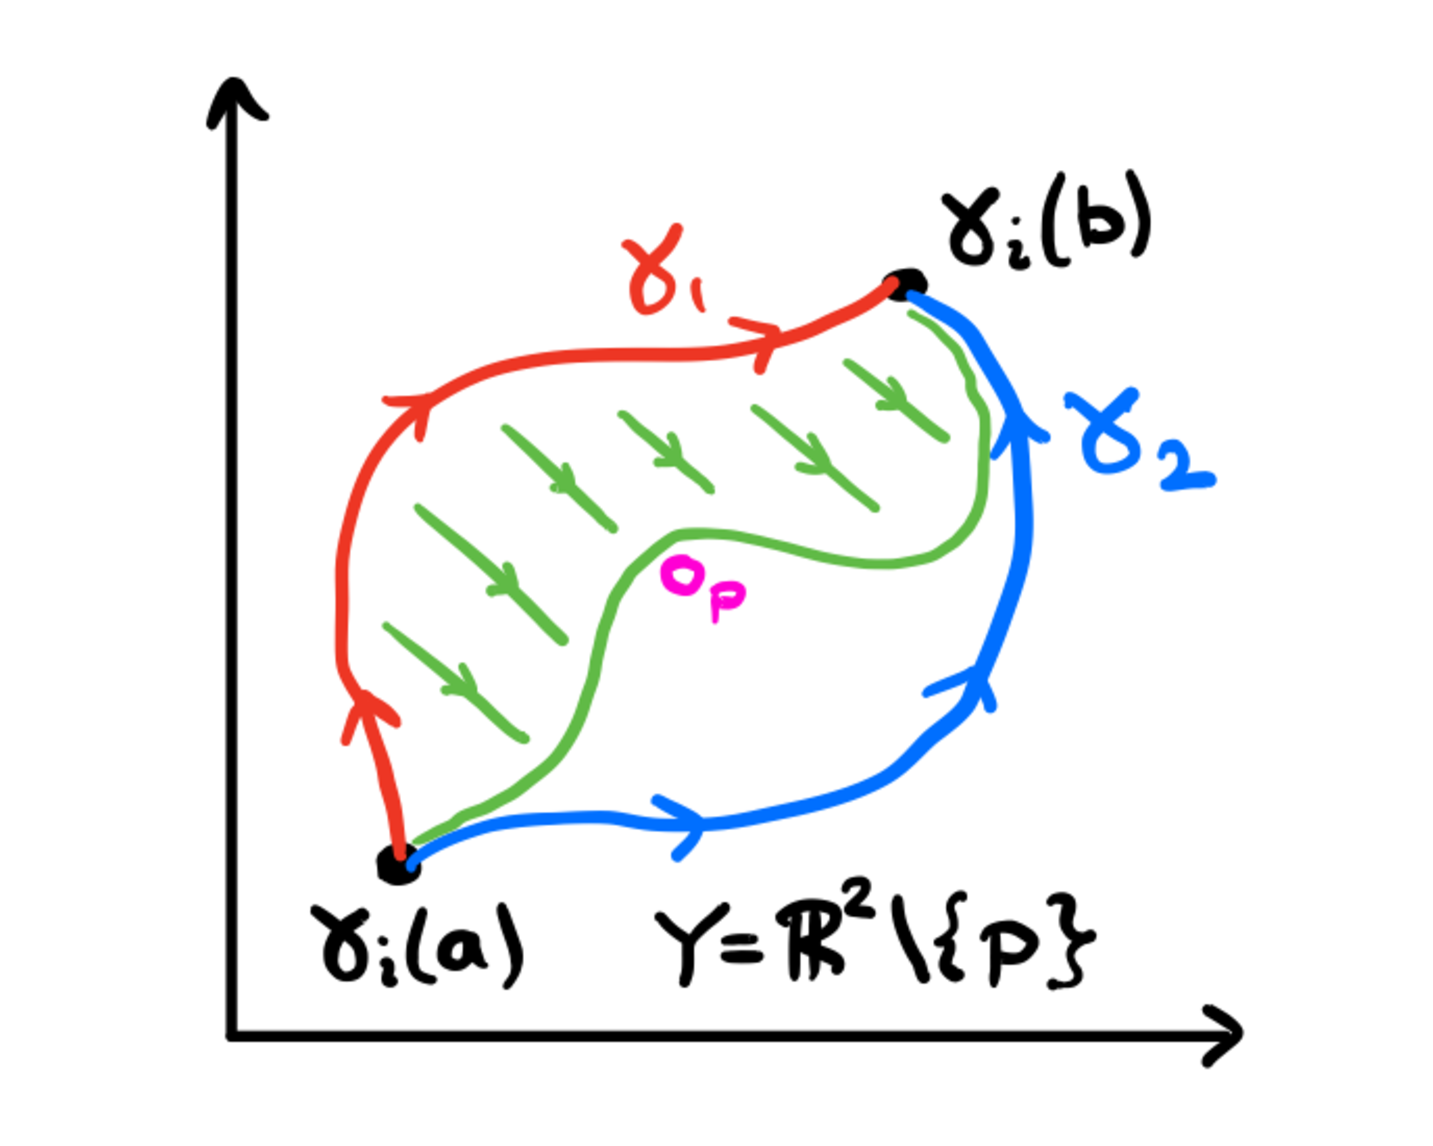
\includegraphics[width = .8\textwidth]{homotopy_2}
		\caption{If $\mathbb R^2$ is punctured, we can no longer deform $\gamma_1$ into $\gamma_2$. }~
		\label{subfig:homotopy2}
	\end{subfigure}~
	\label{fig:homotopy}
	\end{figure}
	\begin{flushleft} \setlength{\parindent}{2em}
	This brings us to the discussion of homotopy groups. We can put a relation $\sim$ on maps $X\rightarrow Y$ by demanding 
	that $f\sim g$ iff $f$ and $g$ are homotopic. It is easy to prove this is an equivalence relation, so we can quotient out by $\sim$. 
	We can furthermore give each equivalence class a group structure by concatenation, i.e. if $[\alpha]$ and $[\beta]$ are 
	equivalence classes of maps with common starting and ending points (loops), then $[\alpha]\cdot[\beta] := [\alpha\cdot\beta]$ is a map which 
	does $\alpha$ first, then does $\beta$. When $X$ is the n-sphere $S^n$, we call the homotopy classes of loops $S^n\rightarrow X$ equipped 
	with this group multiplication the \textbf{n$^th$ homotopy group of $X$}, and denote it by $\pi_N(X)$. 
	
	As an example, $\pi_1(\mathbb R^2) = 0$ because every loop can be continuously deformed into every other loop. However, if we look 
	at the punctured plane, $\pi_1(\mathbb R^2\setminus \{(0, 0)\}\cong\mathbb Z$. A map which winds around the puncture $n$ times cannot 
	be deformed into a map which winds around the puncture $m$ times; to create a homotopy between these loops, we would need to 
	pass over the puncture, which we cannot do continuously. In the same way, we have the fundamental relation:
	\begin{equation}
		\pi_1(S^1)\cong\mathbb Z
	\end{equation}
	The $n^{th}$ homotopy class is generated by the map with winding number $n$, $e^{i\theta}\mapsto e^{in\theta}$. 
	\end{flushleft}
\end{answer}

\newpage
\section{Instantons in QM}

This section will examine how instantons arise in a regular 1D quantum mechanical theory; it will rely heavily on Sydney Coleman's 
lectures on symmetry~\cite{coleman_instantons}, Ch. 7. We will study the three potentials depicted in 
Figure~\ref{fig:instanton_potentials}. The first potential is just a simple harmonic oscillator, which will 
give us a glimpse of how a free theory behaves. The second potential is a double well, and it is here we will see the first example of 
instantons; these will be classical trajectories moving us from one well to the other. Finally, we will briefly look at a periodic potential, 
which is sometimes called an instanton gas. 
\begin{figure}[H]
	\centering
	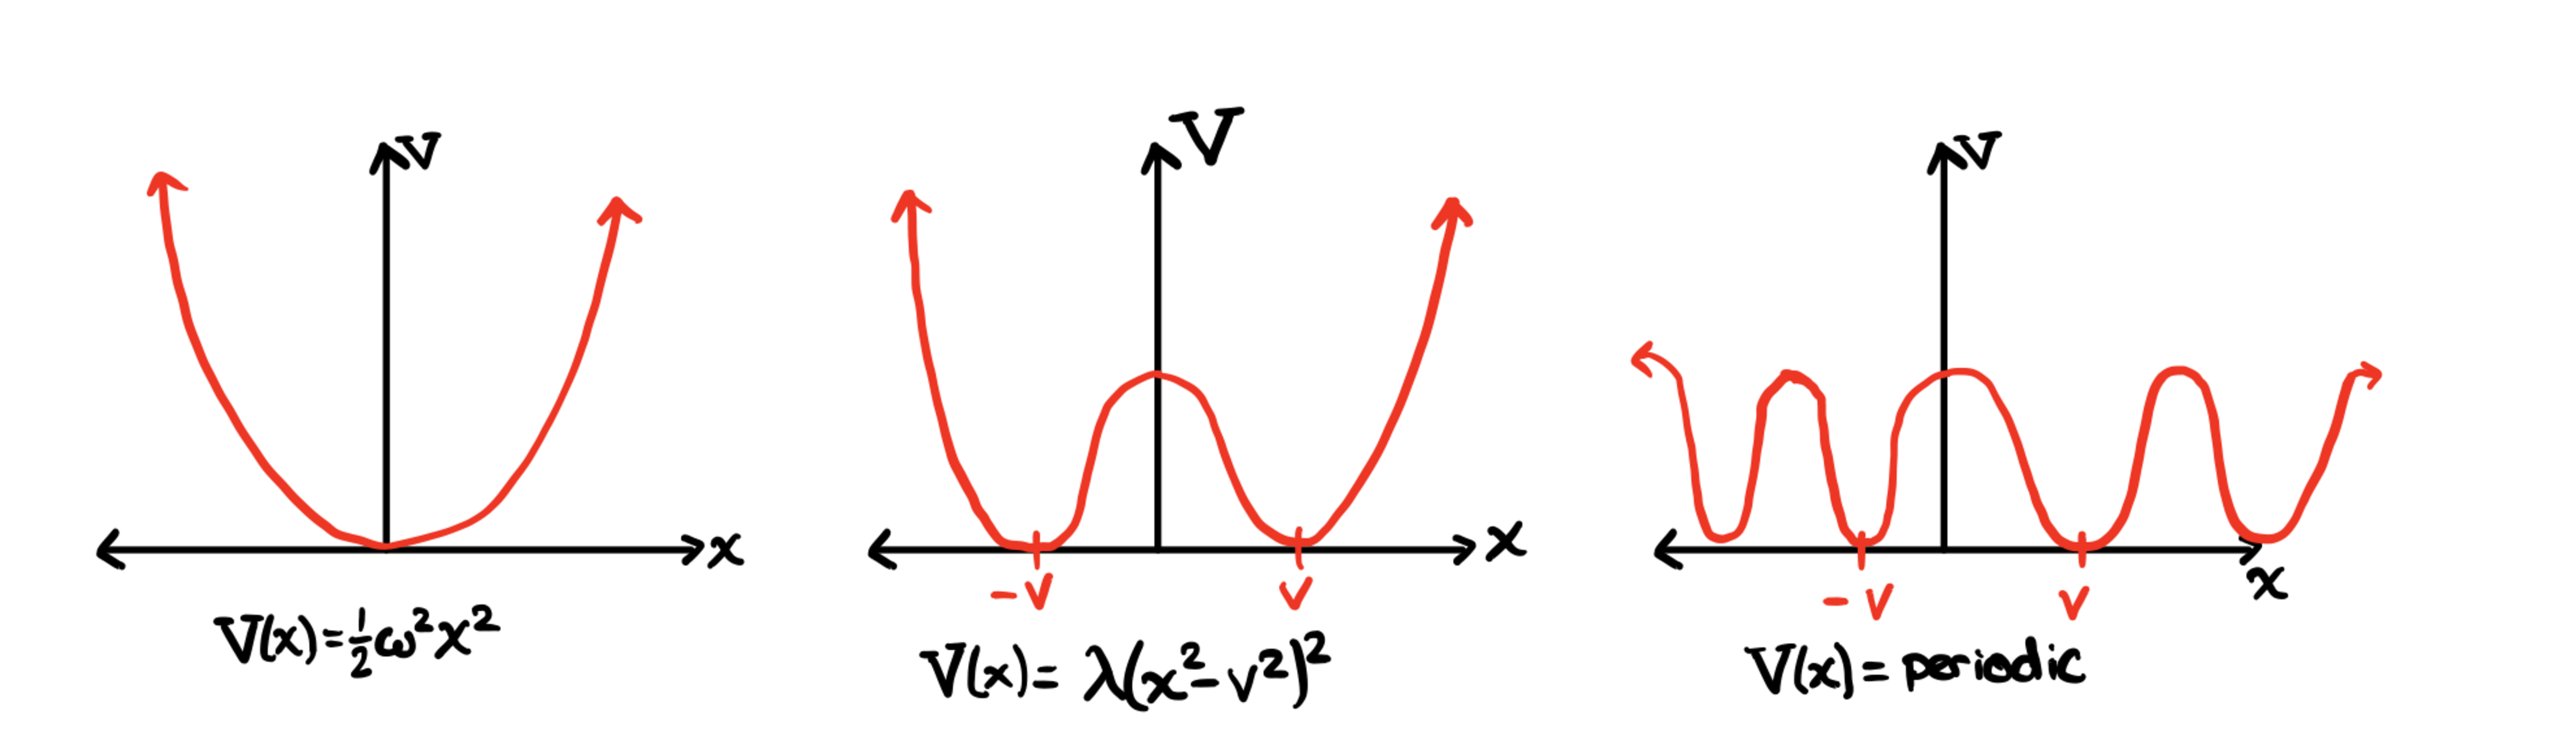
\includegraphics[width = .9\textwidth]{instanton_potentials}
	\caption{Potentials of interest: a harmonic well, a double well, and a periodic potential.}~
	\label{fig:instanton_potentials}
\end{figure}
Some of the features will be quite similar to the 1D soliton solution we discussed above, because we we will be using the same 
generic type of potential. The differences between this example and the previous one is the dimensionality of the configurations we are looking at. 
In the soliton case, we considered a field in a (1 + 1)d theory, since we looked at the soliton as a time-independent classical solution 
which is localized in space. In this section, we consider instantons in QM: these are no longer time-independent solutions and are 
occuring in a (0 + 1) dimensional spacetime (i.e. quantum mechanics). The essential machinery that we will use is about the same, 
but the setups are subtly different. 

To begin, we will compute the Euclidean transition amplitude
\begin{equation}
	\langle x_f | e^{-HT / \hbar} | x_i\rangle = \int Dx e^{-S[x] / \hbar}~
	\label{eq:shm}
\end{equation}
for the simple harmonic oscillator using the principal of steepest descent. Recall steepest descent tells us that for an exponentially decaying 
integral like Eq.~(\ref{eq:shm}), the primary contribution to the integral will come from a stationary point $X(t)$ (we will assume there is only 
one for now) of the action, i.e. $\delta S|_{X} = 0$, multiplied by a characteristic width around this stationary point. The stationary point 
can be obtained by varying the action, and the width from solving for the deviation up to quadratic order about the 
stationary point:
\begin{align}
	- \partial_t^2 X + V'(X) = 0 && - \partial_t^2x_n + V''(X) x_n = \epsilon_n x_n~
	\label{eq:eigenvalue_shm}
\end{align}
Note here that \textit{the stationary point solves the Euler-Lagrange equations for the potential of $-V(x)$ (the minus is due to the Wick rotation 
to move us to Euclidean space) and thus $X(t)$ is a solution to the classical equations of motion in the potential $-V(x)$}. This is a general 
feature and will allow us to analyze instanton solutions with our intuition from classical mechanics. Mathematically, these solutions are 
combined into the equation:
\begin{equation}
	\langle x_f | e^{-HT / \hbar} | x_i\rangle \sim N e^{-S[X]} \prod_n \epsilon_n^{-\frac{1}{2}} = Ne^{-S[X]} \det\left(-\partial_t^2 + 
	V''(X)\right)^{-\frac{1}{2}}~
	\label{eq:instanton_qm}
\end{equation}
where $\sim$ denotes equality up to order $\mathcal O(\hbar)$, $N$ is some normalization, and we use that the determinant of an operator 
is the product of its eigenvalues. 

Since the negative potential is the one which appears in the Euclidean EoM, we sketch the negative potentials in 
Figure~\ref{fig:negative_potentials}. 
\begin{figure}[H]
	\centering
	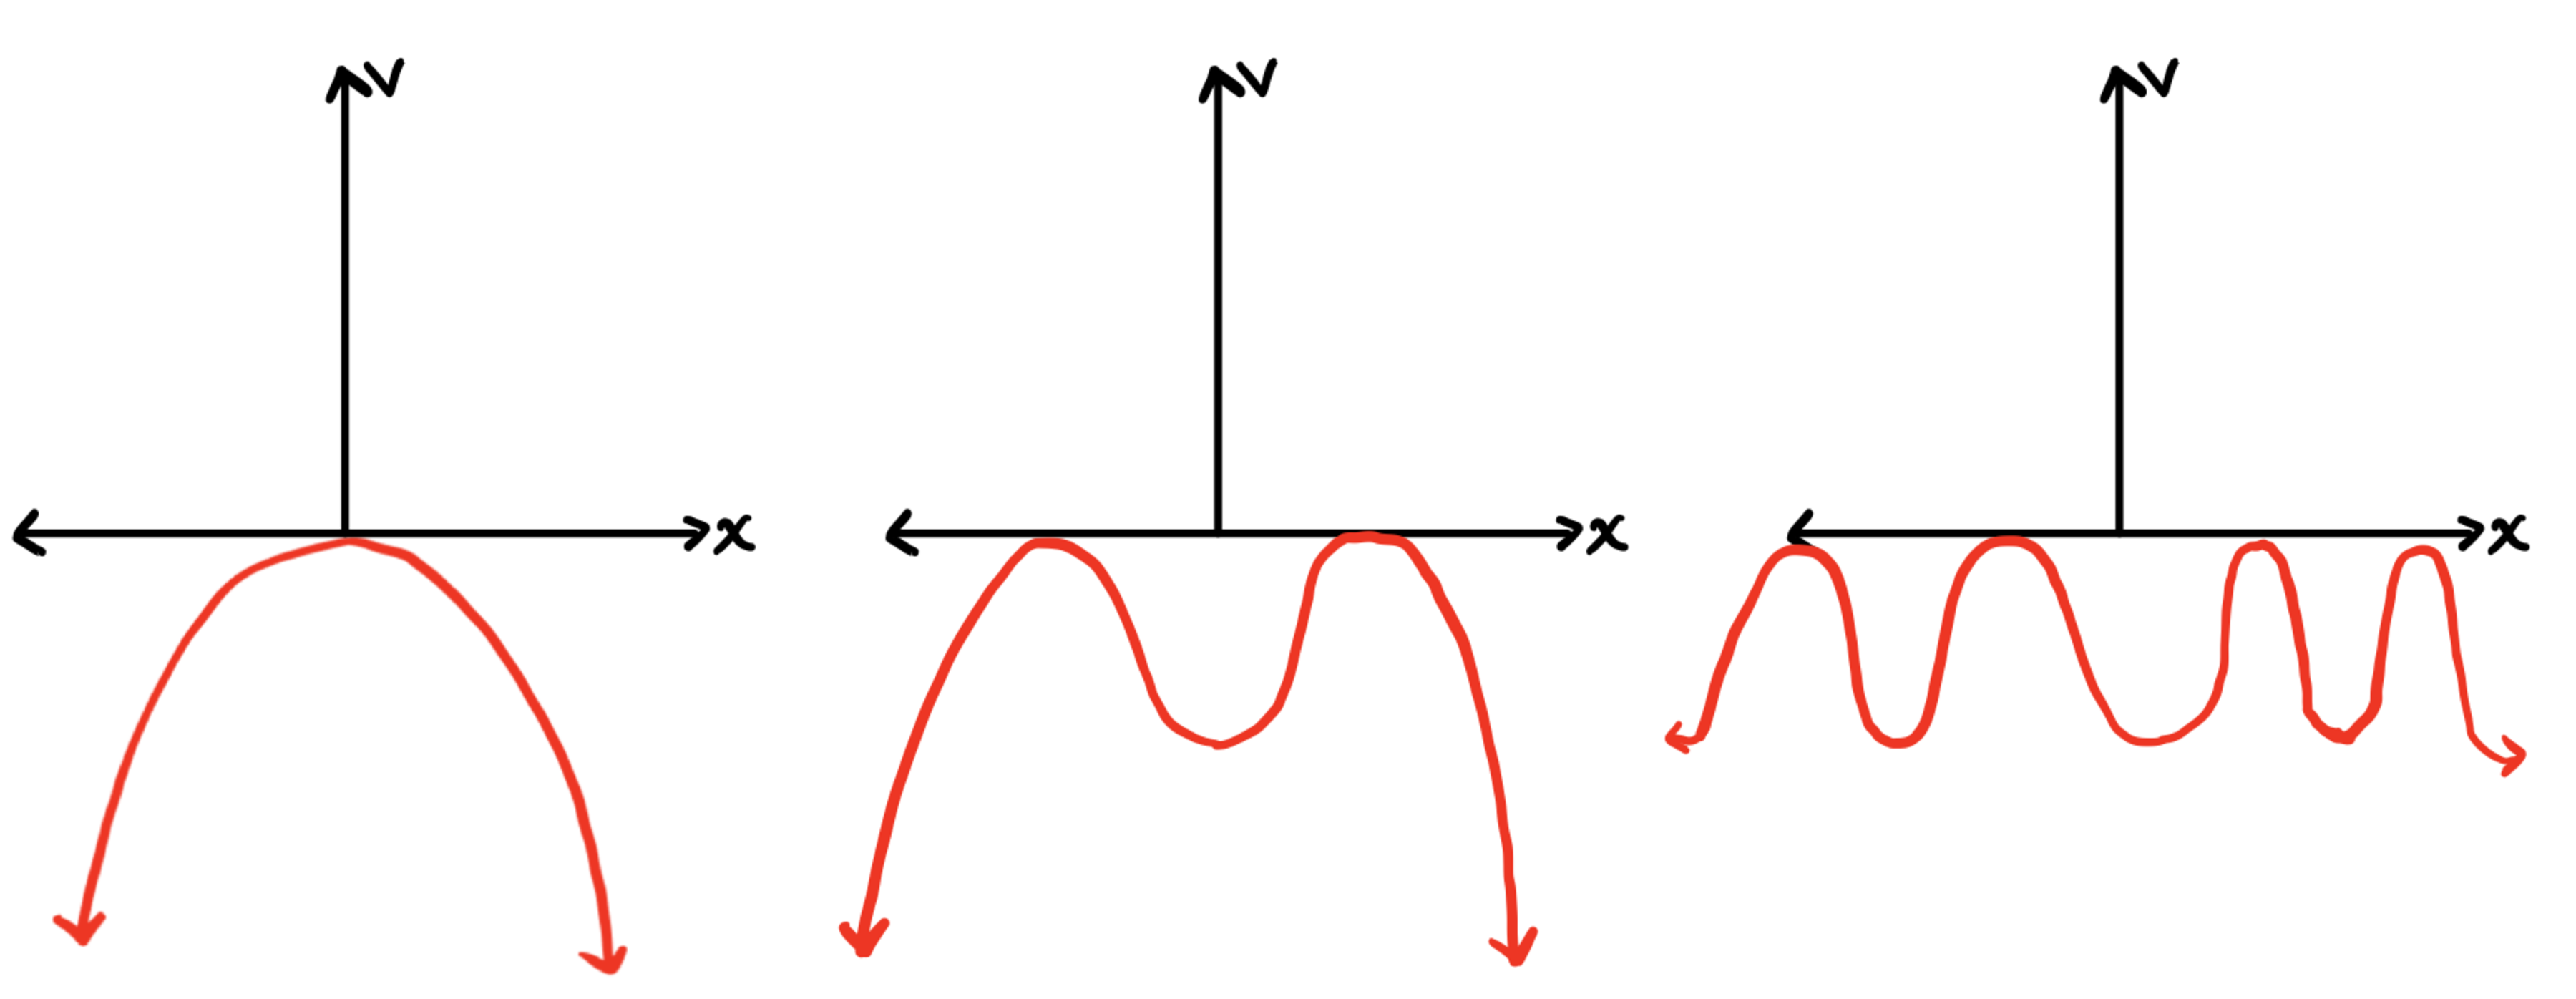
\includegraphics[width = .9\textwidth]{instanton_minus_potentials}
	\caption{Negative of the original potentials $V(x)$, for use in the Euclidean EoM.}~
	\label{fig:negative_potentials}
\end{figure}
We can then determine the classical solutions $X$ by analyzing the classical orbits in the potential $-V(x)$. For the SHM potential, 
there is only one stable solution for $X$: the solution where $X$ is identically 0. In this case, $S[x_0]$ vanishes, and Coleman shows 
that in the $T\rightarrow\infty$ limit, the SHM determinant factor is:
\begin{equation}
	N det(-\partial_t^2 + V''(X)) = \left(\frac{\omega}{\pi\hbar}\right)^{\frac{1}{2}} e^{-\omega T / 2}
\end{equation}
Using this expression in~\ref{eq:instanton_qm} and $S_0 = 0$, we can immediately read off the lowest energy level for the oscillator 
by comparing this solution to the spectral decomposition $\langle x_f | e^{-HT / \hbar} | x_i\rangle \sum_n e^{-E_n T / \hbar} \rightarrow e^{-E_0T / \hbar}$ as 
$T\rightarrow\infty$. This reproduces the correct ground state energy $E_0 = \hbar\omega / 2$; although this process is much more labor 
intensive than the usual methods to compute energy eigenvalues, we will see the advantages it grants us in the double well case. 

Let us now consider the double well potential, $V(x) = \lambda (x^2 - v^2)^2$. The negative of this potential is shown in 
Figure~\ref{fig:negative_potentials}, and like in the SHM case we wish to analyze the classical orbits of $-V(x)$. This case shares some 
similarities with the previous one; we can have two SHM-like solutions where $X \equiv v$ or $X\equiv -v$ and is stationary, or we can 
consider a more intricate solution, where our particle starts at $\pm v$ and rolls along the well, eventually stopping on the other peak at $\mp 
v$. This solution is called the \textbf{instanton solution}. It corresponds to the orbits of the classical field equations which lead to 
tunneling, as we can see since the particle ends on a different hump than it starts on (in Minkowski spacetime without the Wick rotation, this 
solution corresponds to a particle tunneling from one well to the other). We wish to study the instanton solution by determining the matrix element:
\begin{equation}
	\langle v | e^{-HT / \hbar} | -v\rangle
\end{equation}
This corresponds to considering classical trajectories with $X(-T / 2) = -v$ and $X(T / 2) = v$ and taking $T\rightarrow\infty$. There are an 
infinite amount of classical trajectories in this limit, parameterized by a center-time $t_c$:
\begin{equation}
	X(t; t_c) = v \tanh\left(\frac{\omega (t - t_c)}{2}\right)
\end{equation}
The solution starts at $-v$ at $T = -\infty$, crosses the origin at $t_c$ (i.e. $X(t_c; t_c) = 0$), and ends at $v$ at $T = \infty$. The $T\rightarrow\infty$ 
limit is the reason that we have an infinite amount of solutions to the equations of motion; this time translation invariance will result in some of the 
topological events we will see. The solution $X(t; t_c)$ is called the \textbf{instanton}, and the opposite solution $X(-t; -t_c)$ which goes from $+v$ to $-v$ 
is called the \textbf{anti-instanton}. By evaluating $S[X]$, we arrive at the \textbf{instanton action}:
\begin{equation}
	S_\mathrm{instanton} = S[X] = -\frac{\omega^3}{12\lambda}
\end{equation}
We see here the first evidence of non-perturbative effects: in Eq.~(\ref{eq:instanton_qm}), the factor of $e^{-S[X]}$ \textbf{will not be 
detected to any order in perturbation theory, since $e^{1/\lambda}$ is not an analytic function}. This means no amount of diagrams will ever 
generate this term, and it cannot be detected by perturbation theory. 

The full one-instanton solution to the double well is a bit more complicated to derive, but is described in Section 3 of~\cite{instanton_abc}. 
The solution is (with $\hbar = 1$ here):
\begin{equation}
	\langle -v | e^{-HT} | v\rangle_\mathrm{1-instanton} = \left(\sqrt{\frac{\omega}{\pi}} e^{-\omega T / 2}\right)\left(\sqrt{\frac{6}{\pi}}\sqrt{S[X]} e^{-S[X]}\right) \omega dt_c
\end{equation}
The factor $K$ is introduced to clean up future expressions; $K^n$ is proportional to the density of instantons. A few notes about this:
\begin{enumerate}
	\item This solution is general except for the prefactor of $\sqrt{6 / \pi}$ which appears from the determinant of the differential operator in 
	Eq.~(\ref{eq:instanton_qm}). We will see the general structure again when we consider the BPST instanton in QCD. 
	\item The $dt_c$ is a remnant of the fact that the operator determinant $det(-\partial_t^2 + V''(X))$ is zero, because the operator has a 
	zero eigenvalue. This zero eigenvalue comes from the translational invariance; we can shift the classical solutions in $t_c$ and still 
	retain a stationary point of the action, so the eigenvalue equation for $\epsilon_n$, Eq.~(\ref{eq:eigenvalue_shm}), has a solution with 
	$\epsilon_n = 0$. Since the full expansion has a factor of $\prod \epsilon_n^{-1/2}$, evaluating the full path integral is formally infinite. 
	So, we instead suppress the integration over the zero mode in the path integral and leave the integral explicit. The integration measure 
	we are leaving unevaluated is $\sqrt{S[X]} dt_c$, which is where those factors appear. 
	\item The first piece of the equation in parentheses is the contribution from the free theory; you can see this because it looks like the 
	SHM path integral for large $T$. The second piece is called the \textbf{instanton density}, and it is the number of instantons / 
	anti-instantons that we see per unit time:
	\begin{equation}
		d = \sqrt{\frac{6}{\pi}}\sqrt{S[X]} e^{-S[X]}
	\end{equation}
	As mentioned before, the prefactor is potential-dependent, but the rest of the structure is quite general. 
\end{enumerate}

Now, we can construct solutions to the classical EoM which incorporate many instantons and anti-instantons instead of just one. 
The idea here is that \textit{instantons are localized in time}, and that the main contribution to the instanton comes over a finite timescale 
$\delta\tau$ (outside of the interval $(t_c - \frac{1}{2}\delta\tau, t_c + \frac{1}{2}\delta\tau)$, $X(t)$ is approximately constant and about 
equal to $\pm v$). So, we can construct \textit{approximate solutions to the equations of motion} if we insert instantons that are well 
separated in time, with $t_\mathrm{sep} >> \delta\tau$. If we are looking at a large timescale $T$ (and we are, since we're taking the 
$T\rightarrow\infty$ limit), which is much larger than the dynamic timescale of each instanton, we can then ``sprinkle in" many instantons to 
create a new classical solution for our theory. As depicted in Figure~\ref{fig:many_instantons}, we can have contributions to the amplitude 
$\langle v | e^{-HT} | -v\rangle$ which correspond to moving from the left well to the right well (one instanton), moving back from the right to 
left well (one anti-instanton), and continue this pattern as many times as we like, as long as asymptotically our solution satisfies 
$X(T\pm\rightarrow\infty) = \pm v$. One can then construct the total instanton contribution to the tunneling amplitude by summing on 
instanton / anti-instanton insertions, and derive an explicit formula for this amplitude-- if you are interested, see Coleman's notes. For now, 
I will just state what the solution looks like, after summing on instanton / anti-instanton insertions:
\begin{equation}
	\langle\pm v | e^{-HT} | -v\rangle  = \frac{1}{2}\sqrt{\frac{\omega}{\pi}} e^{-\omega T / 2} \left[\exp\left( K e^{-S_0} T \right) \mp \exp\left( -K e^{-S_0} T \right)\right]
\end{equation}
where $K$ is a constant which can be related to the one-instanton solution. 

\begin{figure}[H]
	\centering
	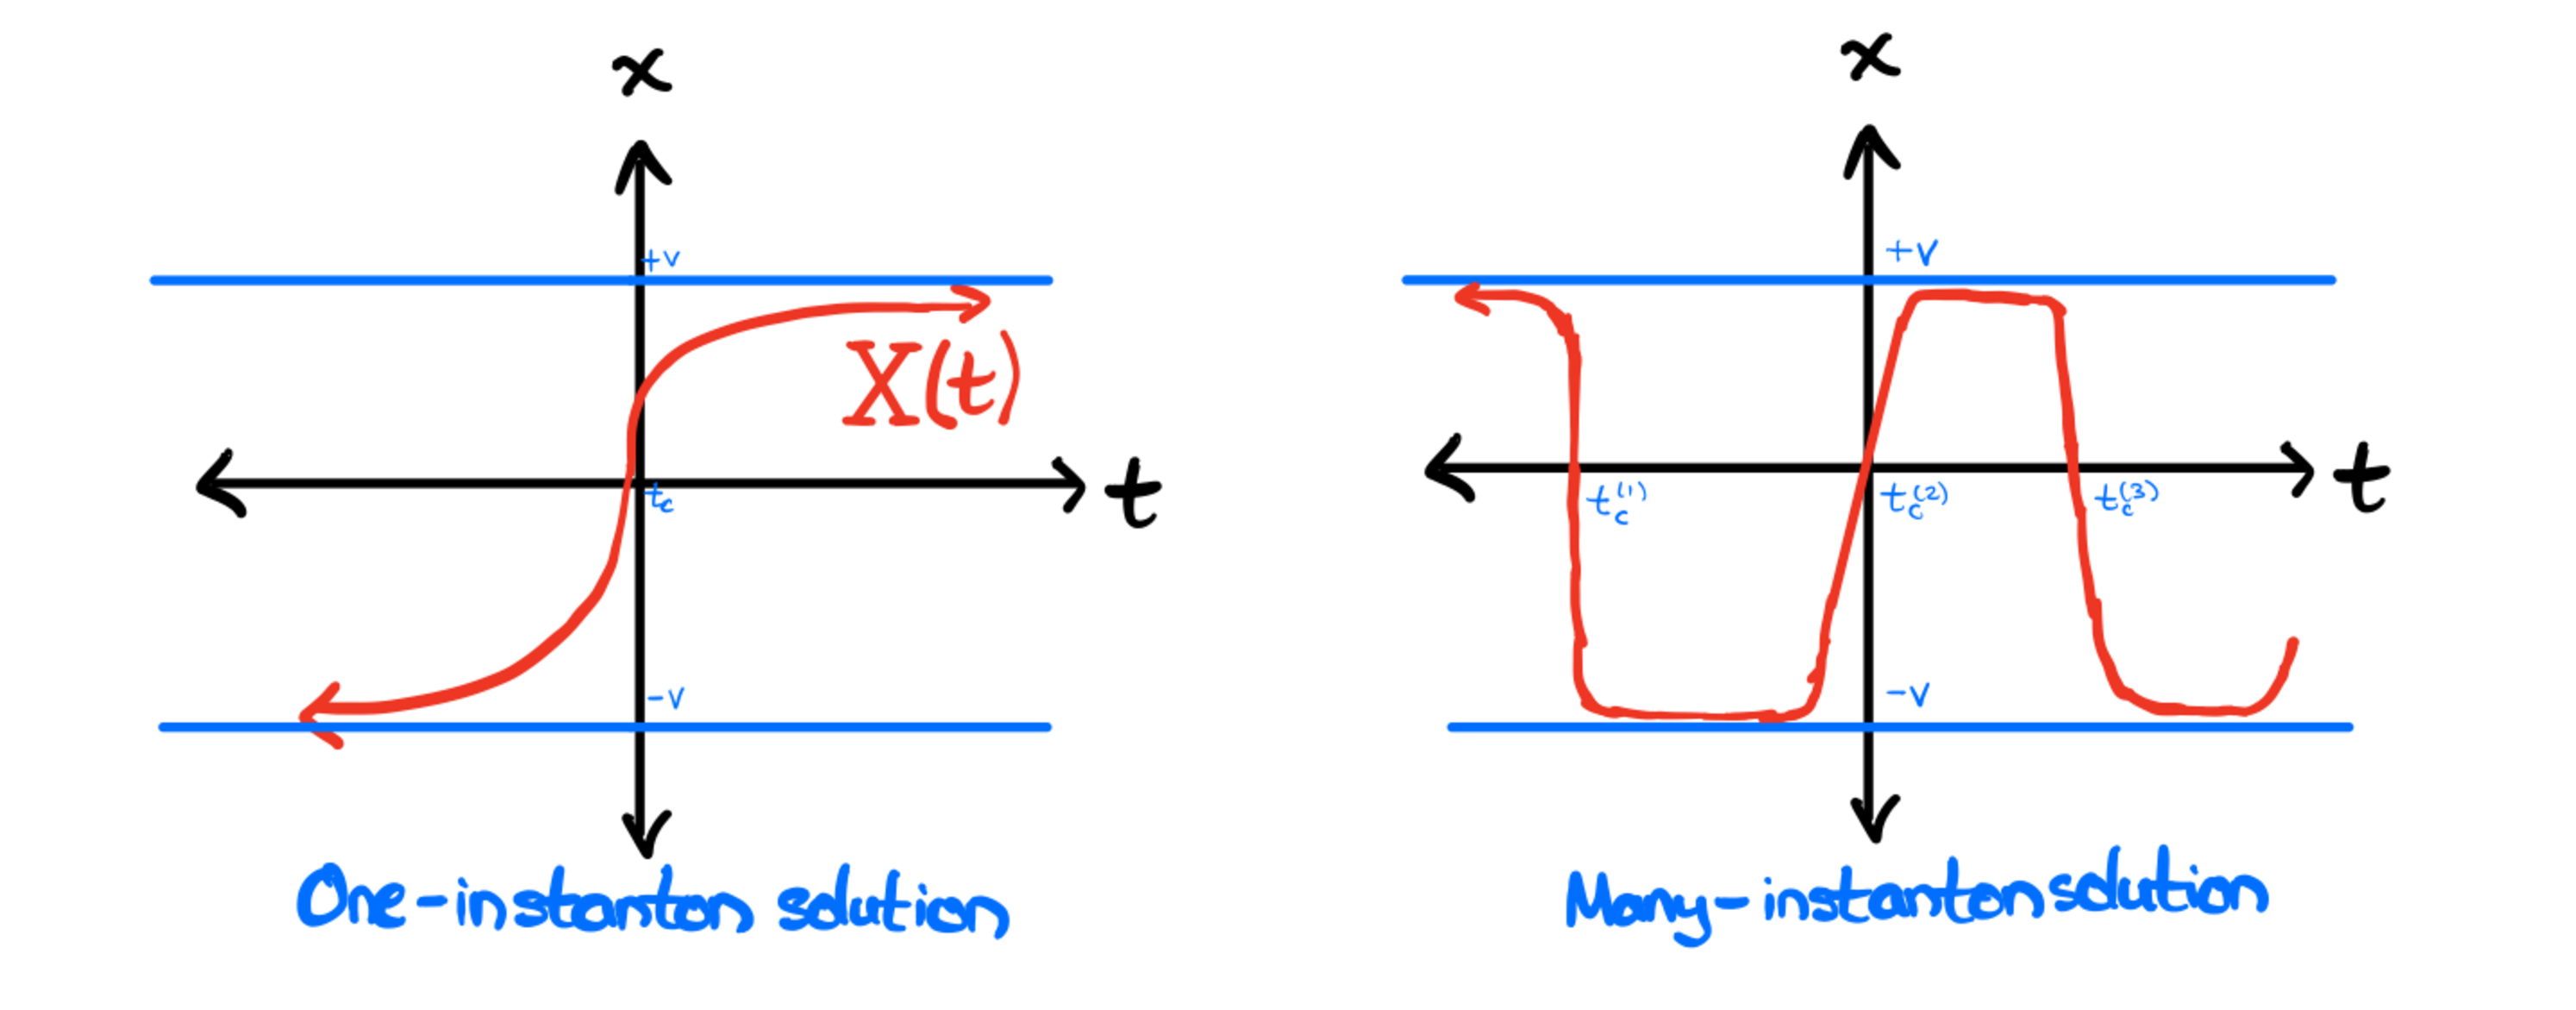
\includegraphics[width = .9\textwidth]{many_instanton_soln}
	\caption{Single and many instanton solutions to the EoM. }~
	\label{fig:many_instantons}
\end{figure}

Finally, we should mention the last potential of interest: the case of a periodic potential. This is the setting for what is called a \textbf{dilute 
instanton gas} (I'm not really sure why). Quantitatively one can determine the one-instanton contribution much like in the 
double-well case. The difference for this potential is that because it is periodic everywhere, when looking at the matrix element 
$\langle mv | e^{-HT} | -nv\rangle$, one must consider an arbitrary path from $-nv$ to $mv$. In the double well case, we could only have 
alternating instanton / anti-instanton contributions, since $X(t)$ has to be connected. In this case, we can have instanton 
contributions from $kv$ to $lv$ for any integers $k, l\in\mathbb Z$, as long as in the infinite time limit they end up at $\pm v$ to satisfy 
the correct boundary conditions. 

The periodic potential will provide some insight into the definition of the $\theta$ vacuum that we will see later for gauge theories. 
If we let $j_-$ and $j_+$ be two minima of the potential, we can construct the tunneling amplitude by summing up all strings of 
instantons which connect $|j_-\rangle$ with $|j_+\rangle$. This gives us (where $n$ and $\overline n$ are the numbers of instantons and 
anti-instantons, and each instanton / anti-instanton takes us plus or minus one well, respectively):
\begin{equation}
	\langle j_+ | e^{-HT} | j_-\rangle = \sqrt{\frac{\omega}{\pi}} e^{-\omega T / 2} \sum_{n = 0}^\infty \sum_{\overline n = 0}^\infty \frac{1}{n!\overline n!} 
	(K e^{-S_0} T)^{n + \overline n}\delta_{j_- + n, j_+ + \overline n}
\end{equation}
Now, the idea is that we would like to find the energy eigenstates of this potential. We will do this by expanding $\langle j_+ | e^{-HT} | j_-\rangle$ into a 
spectral decomposition; we will cast it as a sum or integral of $e^{-E(\phi) T}|N(\phi)$, where $|\phi\rangle$ are our energy eigenstates. 
We accomplish this by expanding $\delta_{ab} = \frac{1}{2\pi}\int_0^{2\pi} d\theta\, e^{i\theta(a - b)}$. Plugging this into the previous equation, we arrive at the 
desired decomposition:
\begin{equation}
	\langle j_+ | e^{-HT} | j_-\rangle = \sqrt{\frac{\omega}{\pi}} e^{-\omega T / 2} \int_0^{2\pi} \frac{d\theta}{2\pi} e^{i(j_- - j_+)\theta}\exp\left(2KT\cos\theta e^{-S_0}\right)~
	\label{eq:1d_theta_vacuum}
\end{equation}
This allows us to see the spectrum of the periodic potential. There is a continuous set of energy eigenstates labeled by $\theta\in [0, 2\pi)$, and each 
state $\theta\rangle$ has energy:
\begin{equation}
	E(\theta) = \frac{1}{2}\omega + 2 K\cos\theta e^{-S_0}
\end{equation}
We can even determine the energy eigenstates by inserting a resolution of the identity with $|\theta\rangle\langle\theta |$ into Eq.~(\ref{eq:1d_theta_vacuum}). 
We see that:
\begin{equation}
	|\theta\rangle = \sqrt{\frac{\omega}{\pi}}\frac{1}{2\pi} \sum_j e^{ij\theta}|j\rangle
\end{equation}
We are going to see an expression resembling this again very soon when we discuss the QCD vacuum. Indeed, this toy model has many of the same 
features the possible QCD vacuum states. Our energy eigenstates are a Fourier transform in $j$ over the distinct topological vacuum states $|j\rangle$. 
We can enumerate these eigenstates with the continuous parameter $\theta$, and the energy has a sinusoidal dependence on $\theta$. 

\begin{answer}
	\begin{center}
		\textbf{Interlude 2: Differential forms and gauge theories}
	\end{center}
	\begin{flushleft} \setlength{\parindent}{2em}
	Differential forms are the language of physics. They provide an elegant formalism to study gauge theories and whenever the topology 
	of gauge theories is discussed, differential forms naturally come into play. Let $\mathfrak{X}(M)$ be the set of vector fields on a 
	$n$-dimensional manifold $M$, so if $X\in \mathfrak{X}(M)$ is a vector field, then at each $p\in M$, $X|_p\in T_p M$ is a vector at $p$. 
	A \textbf{differential $k$-form} $\phi\in\Omega^k(M)$ is an alternating map which takes in $k$ vector fields and returns a function: 
	you can think of $\phi$ as being a field on $M$ with components $\phi_p$ such that $\phi_p(X_1|_p, ..., X_k|_p)\in\mathbb 
	R$ and $\phi_p(..., X_i|_p, ..., X_j|_p, ...) = $ $-\phi(..., X_j|_p, ..., X_i|_p, ...)$.
	
	A \textbf{connection} on $M$ is a map $\nabla: \mathfrak X(M) \times \mathfrak{X}(M)\rightarrow\mathfrak{X}(M)$ which satisfies the 
	Leibniz rule, $\nabla_X(fY) = (\nabla_X f) Y + f (\nabla_X Y)$. Given a connection, we can define its \textbf{curvature} as the 
	tensor $R : \mathfrak X(M)\times \mathfrak X(M)\rightarrow End(\mathfrak X(M))$, $R(X, Y) Z := \nabla_X \nabla_Y Z - 
	\nabla_Y\nabla_X Z - \nabla_{[X, Y]} Z$. This tensor tells us the amount $\nabla$ fails to 
	preserve the Lie bracket on $\mathfrak X(M)$. Let us pick a orthonormal frame $\{e_1, ..., e_n\}$ (a smoothly-varying ON basis, so 
	$\{e_1|_p, ..., e_n|_p\}\subset T_p M$ is a ON basis for $T_p M$) for the tangent bundle of $M$. Then for each $i, j$, we can define two 
	differential forms of interest: the \textbf{connection form} $(\omega_e)_i^j\in \Omega^1(M)$, and the \textbf{curvature form} 
	$(\Omega_e)_i^j\in\Omega^2(M)$ as follows (this equation holds at each $p\in M$):
	\begin{align}
		\nabla_X e_i =: (\omega_e)_i^j(X)e_j && R(X, Y) e_i =: (\Omega_e)_i^j(X, Y) e_j~
		\label{eq:change_of_frame}
	\end{align}
	$\omega$ is then a $n\times n$ matrix of one-forms, and $\Omega$ is a $n\times n$ matrix of two-forms. Using the relations between 
	$\nabla$ and $R$, one can forms via the second structural equation:
	\begin{equation}
		\Omega_i^j = d\omega_i^j + \omega_i^k\wedge \omega_k^j~
		\label{eq:second_structural}
	\end{equation}
	
	Suppose we change our frame to $\{f_1, ..., f_n\}$ via a unitary matrix $a_i^j(p)$ at each point, so $f_i|_p = e_j|_pa_i^j(p)$. Then it can 
	be shown that $\omega$ and $\Omega$ change accordingly:
	\begin{align}
		\omega_f = a^{-1} \omega_e a + a^{-1} da && \Omega_f = a^{-1} \Omega_e a~
		\label{eq:change_of_frame}
	\end{align}
	If we have a collection of framed open sets $(U, \{e^U_i\}_{i = 1}^n)_U$ covering our manifold with connection / curvature forms 
	$\{(\omega_{e^U})_i^j, (\Omega_{e^U})_i^j\}_U$ satisfying the compatibility conditions, Eq.~(\ref{eq:change_of_frame}), as we move 
	from one patch to another, these locally defined forms \textit{completely define} the connection and the curvature on $M$. 
	Furthermore, the change of frame equation should look familiar to you: this is how the gauge potential $A_\mu$ and field strength 
	$F_{\mu\nu}$ change under gauge transformation:
	\begin{align}
		A_\mu\xrightarrow{U} U^\dagger A_\mu U + U^\dagger \partial_\mu U && F_{\mu\nu}\xrightarrow{U} U^\dagger F_{\mu\nu} U
	\end{align}
	For a gauge theory we are really working with a connection on a principal bundle and not a vector bundle, these are closely 
	related, so we won't deal with the technicalities. Let $\mathcal A$ and $\mathcal F$ be the connection and curvature forms 
	for the principal bundle describing our gauge theory. \textit{Then we can take $\mathcal A = A_\mu dx^\mu$ and $\mathcal F = 
	\frac{1}{2}F_{\mu\nu}dx^\mu\wedge dx^\nu$, and a gauge transformation is just a change in frame}. Furthermore, the second 
	structural equation, Eq.~(\ref{eq:second_structural}) reproduces the usual relation between $F_{\mu\nu}$ and $A_\mu$ (the 
	antisymmetric wedge product on the vector bundle gets lifted to a Lie bracket on the principal bundle):
	\begin{equation}
		F_{\mu\nu} = \partial_\mu A_\nu - \partial_\nu A_\mu + [A_\mu, A_\nu]
	\end{equation}
	
	\end{flushleft}
\end{answer}

\newpage
\section{Solitons}

Let us study solitons a bit more rigorously than in the introduction. Formally, a \textbf{soliton} is a time-independent 
finite-energy field configuration which is a solution to the classical equations of motion. The finite-energy (action) requirement means that 
the energy density of a soliton or instanton is localized in space, and we can treat this lump of energy like a particle. It also implies that as we take $\vec x\rightarrow\infty$, 
$\phi(x)$ must minimize its energy and must approach the vacuum manifold, as we saw in the 1d case where for $x\rightarrow\pm\infty$, 
$\phi(x)\rightarrow \pm v$. Because of this constraint, we can study solitons purely topologically. In a $(d + 1)$ dimensional QFT with vacuum 
manifold $M$, solitons must correspond to maps from the boundary into the vacuum manifold:
\begin{equation}
	S^{d - 1} = \partial\mathbb R^d\rightarrow M
\end{equation}
Solitons can be continuously deformed into one another iff they are homotopic, so to look for distinct soliton solutions to the field equations, 
we are interested in the homotopy group:
\begin{equation}
	\pi_{d - 1}(M)
\end{equation}
Different theories will have different values of $d$ and different vacuum manifolds, so we will study a few examples of this now to gain some 
intuition. Before we begin, we note that with only scalar fields, finding soliton solutions is not usually possible.
\begin{theorem}[Derrick]
	Using only scalar fields, there are no time-independent, finite-energy field configurations which are localized in $> 1$ dimension.
\end{theorem}
This theorem is easily understandable by looking at the two-dimensional example. Consider a complex scalar field $\phi(x)$
in a $(2 + 1)$d spacetime with the standard Mexican hat potential:
\begin{equation}
	V(\phi) = \frac{1}{4}\lambda (\phi^\dagger\phi - v^2)^2
\end{equation}
The classical vacuum manifold $M$ is the set of field configurations which satisfy $|\phi(x)|^2\rightarrow v^2$ as $x\rightarrow\infty$, so we can 
describe $\phi(x)$ as:
\begin{equation}
	\phi(r, \theta)\rightarrow ve^{in\theta}
\end{equation}
as $r\rightarrow\infty$ (since $\pi_1(S^1) = \mathbb Z$, every field configuration on the boundary is homotopic to $e^{in\phi}$, where $n$ is the winding 
number of the configuration). We can thus guess an ansatz for the soliton solution by multiplying this with a function of $r$:
\begin{equation}
	\phi(r, \theta) = v f(r) e^{in\theta}
\end{equation}
where $f(r)\rightarrow 1$ as $r\rightarrow\infty$. To see why Derrick's theorem applies to this example, recall that $\nabla\phi = ve^{in\theta} (f'(r)\hat r + in\frac{f(r)}{r}\hat\theta)$. 
The energy of the field will thus be infinite as we take $r\rightarrow\infty$:
\begin{equation}
	E = \int d^2 \vec x |\nabla\phi|^2 = v^2 \int d^2 \vec x \left[ f'(r)^2 + n^2 \left(\frac{f(r)}{r}\right)^2\right]\xrightarrow{r\rightarrow\infty} v^2 n^2 \int_0^\infty dr\frac{f(r)^2}{r} = \infty
\end{equation}
This behavior can be shown to be general in $\geq 2$ spatial dimensions, because the measure $d^n\vec x = r^{n - 1} dr d\Omega$, 
and for $n \geq 2$ this $r^{n - 1}$ term will dominate the integral and cause a divergence for $n\neq 0$. 

So, where do we go from here to study more interesting topological features? We can look at gauge theories. These will be different than 
theories with just a scalar field because in a gauge theory, the kinetic energy term will use a covariant derivative instead of an 
ordinary derivative:
\begin{equation}
	\int d^n\vec x \, |D_\mu\phi|^2 = \int d^n\vec x \,|(\partial_\mu - ig A_\mu)\phi |^2
\end{equation}
We can thus pick gauge field configurations which make this term finite as $r\rightarrow\infty$. For the previous case, we will promote the 
global $U(1)$ symmetry to a gauged $U(1)$ theory. Then to make the energy finite, we must have $|D_\mu \phi|^2\rightarrow 0$ \textit{faster than 
$\frac{1}{r^2}$ as $r$ tends towards infinity}. That is, we can take:
\begin{equation}
	A_\mu = -\frac{i}{gv^2}\phi^\dagger \partial_\mu\phi + \mathcal O\left(\frac{1}{r^2}\right)\xrightarrow{r\rightarrow\infty} \frac{1}{g}\frac{n}{r}\hat\theta
\end{equation}
The first term is \textbf{pure gauge}; it is locally a gauge transformation of the trivial field configuration, since $A_\mu\mapsto U^\dagger A_\mu U + U^\dagger 
\partial_\mu U$ under gauge transformation. Adding in a term that is pure gauge is sufficient to cancel out the diverging behavior of $\partial_\mu\phi$ as 
$r\rightarrow\infty$, as long as there is no $r$ dependence in $A_\mu$ which will cause further divergences. 

% U(1) gauge theory in 2d
To study these soliton solutions, we are really just looking at what $A_\mu$ can look like on the boundary of spacetime. In two spatial dimensions, 
$\partial\mathbb R^2\cong S^1$, so we are looking at for continuous fields on $S^1$ which are valued in $U(1)$ (these are the same manifolds, 
I am just using different notation for conventional purposes). These fields are characterized by their \textbf{winding number} $\nu$, which is equal to their 
homotopy class. An explicit formula for this is given by evaluating the circulation integral at the boundary of space:
\begin{equation}
	\nu = \frac{g}{2\pi} \int_{S^1(r\rightarrow\infty)} ds^\mu A_\mu = \frac{g}{2\pi} \int_0^{2\pi} d\theta\, r\frac{n}{gr} = n
\end{equation}
Fields which live in the same homotopy class \textit{can be deformed into one another with a finite amount of energy; field configurations which live in distinct 
homotopy classes cannot}. This is depicted pictorially below: the maps we are interested in can be depicted by unit vector fields 
living on a circle.

\begin{figure}[H]
	\centering
	\begin{subfigure}[t]{.4\textwidth}
		\centering
		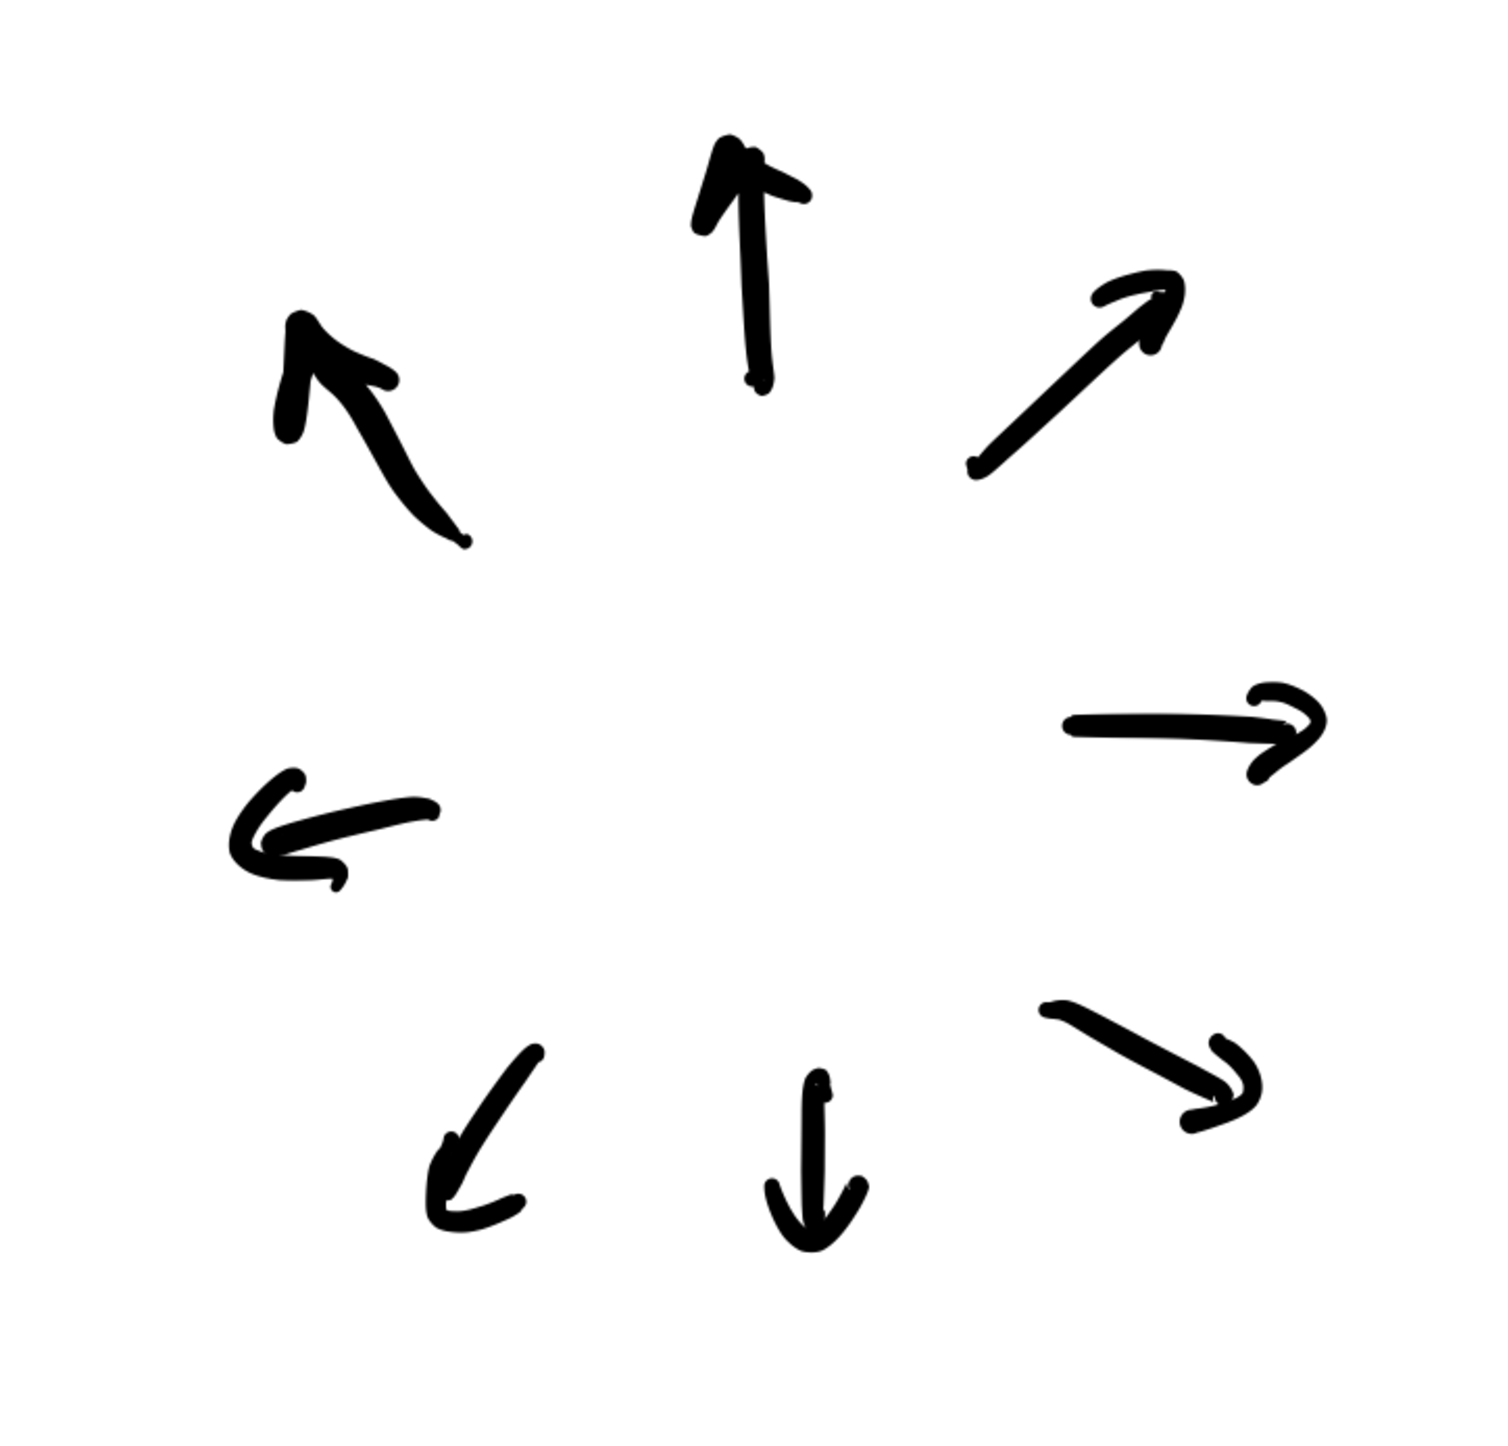
\includegraphics[width = .8\textwidth]{soliton_one_wind}
		\caption{Configuration with winding number $\nu = 1$.}~
		\label{subfig:one_wind}
	\end{subfigure}
	~
	\begin{subfigure}[t]{.4\textwidth}
		\centering
		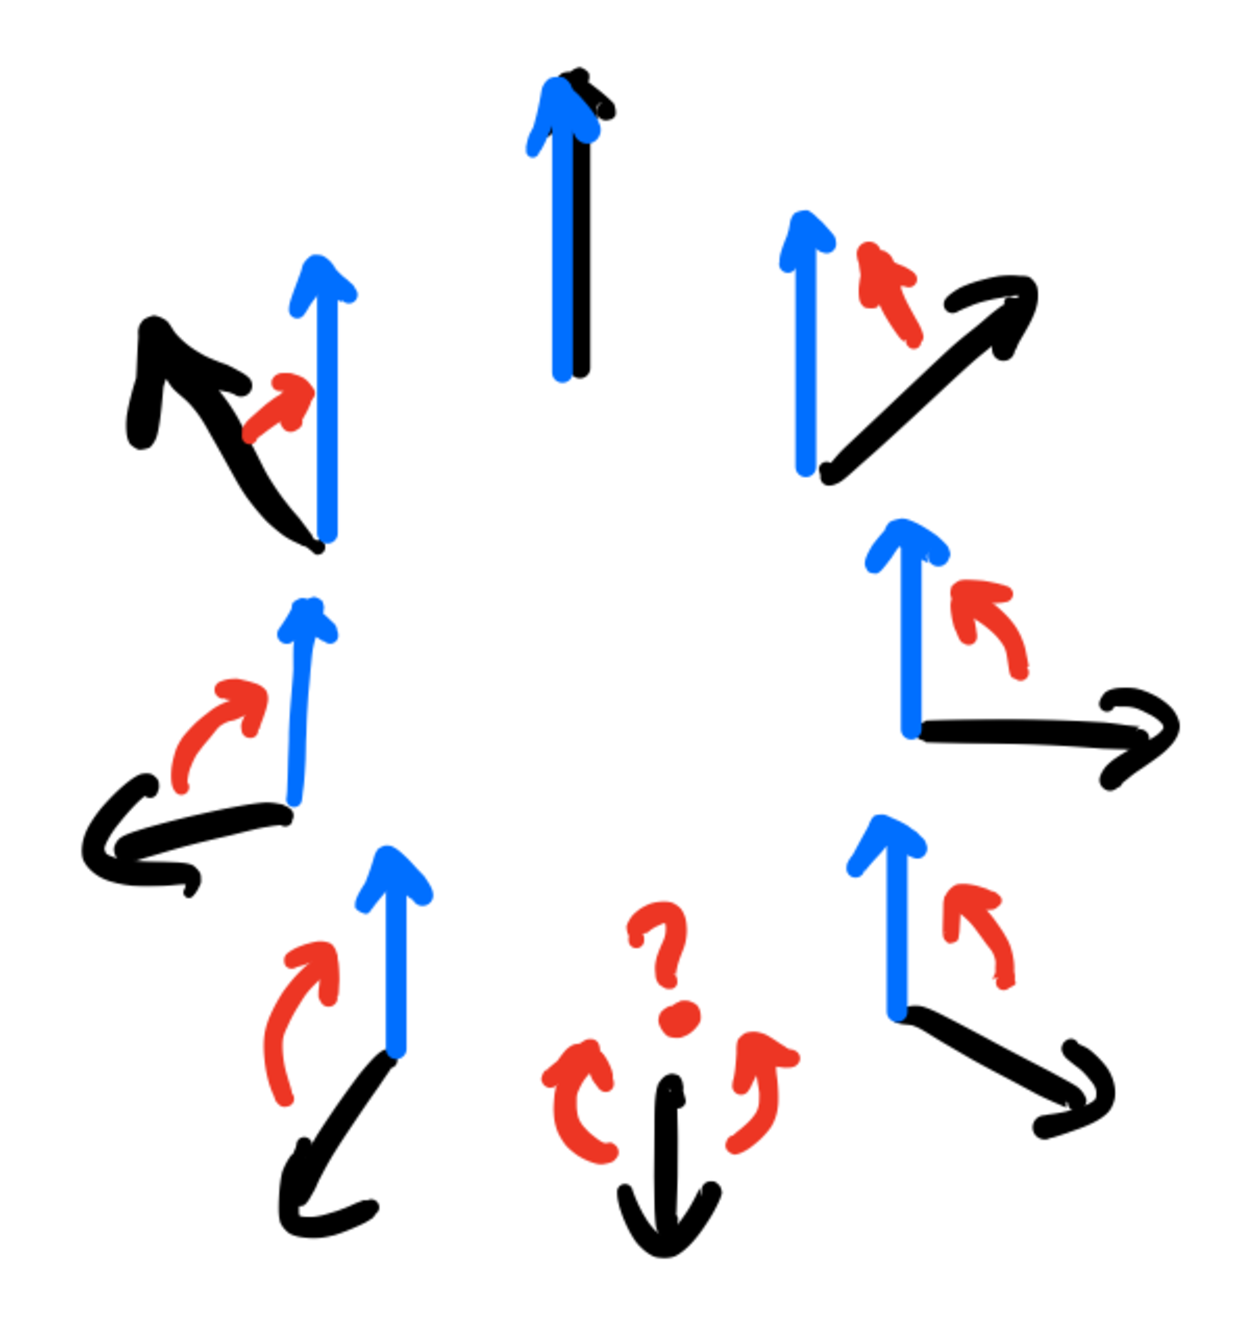
\includegraphics[width = .8\textwidth]{soliton_trivial}
		\caption{Attempt to deform $\nu = 1$ configuration into a trivial $\nu = 0$ configuration. }~
		\label{subfig:trivial}
	\end{subfigure}~
	\label{fig:deformation}
\end{figure}

The original field in Figure~\ref{subfig:one_wind} has winding number 1, and we wish to deform this continuously into a field with winding 
number 0, which in this case will have arrows pointing straight up. As shown in Figure~\ref{subfig:trivial}, we can rotate most of the black 
arrows into blue arrows without problem; however, there will always be one point at which we are unable to continue performing this 
continuously. At the bottom point in the figure, we can either rotate the original vector left or right; if we rotate it left, it will be discontinuous on 
the right, and vice versa if we rotate it to the right. This is a direct consequence of $\pi_1(S^1) = \mathbb Z$; these two configurations 
are not in the same homotopy class, and hence cannot be deformed into one another. 

\newpage
\section{Instantons in QFT}
% Instantons with an SU(2) theory
This pure gauge term is more general than just for the $U(1)$ theory. Suppose we have a pure gauge theory in $D = d + 1$ Euclidean 
dimensions with gauge group $G$. An \textbf{instanton} is a field configuration in Euclidean spacetime with a finite action.  
Instantons will appear in processes like tunneling, because in tunneling we are interested in probabilities to tunnel between different 
vacuum states as a function of time. For the instanton to have a finite action, we need the field configuration to approach the vacuum 
manifold as we take $T\rightarrow\pm\infty$, and as we have already discussed many times, the distinct gauge field configurations that 
the instanton can approach at $\pm T$ are given by the homotopy classes of $G$. 

Asymptotically, $A_\mu$ must decay so that $\int tr[F_{\mu\nu} F^{\mu\nu}]$ becomes finite. This means that any radial dependence of 
$F_{\mu\nu}$ must decay faster than $\frac{1}{r^2}$, so $A_\mu$ must have no dependence on $r$ which is stronger than $\frac{1}{r^2}$. 
However, $A_\mu$ can have angular dependence on top of this behavior in $r$, as long as $F_{\mu\nu}$ vanishes. This means that 
$A_\mu$ must be pure gauge up to order $\frac{1}{r^2}$, and so we have the same expression as in the $U(1)$ case:
\begin{equation}
	A_\mu = g \partial_\mu g^\dagger + \mathcal{O}\left(\frac{1}{r^2}\right)~
	\label{eq:pure_gauge}
\end{equation}
where here $g : S^3\rightarrow G$ is an angular field with values in $G$. Under a gauge transformation $U(x)\in G$, we see that:
\begin{equation}
	A_\mu\mapsto (Ug)\partial_\mu (Ug)^\dagger + \mathcal O\left(\frac{1}{r^2}\right)
\end{equation}
so Eq.~(\ref{eq:pure_gauge}) still holds with $g\mapsto Ug$. If we can take $U = g^\dagger$, we can eliminate this pure gauge term 
entirely. Unfortunately, hOmOtOpY says we cannot always do that. $U(x)$ must be a global gauge transformation, and hence a continuous 
map $U : \mathbb R^4\rightarrow G$. If $g$ is not homotopic to the identity, then we cannot extend $g^\dagger$ to a global field on all of $\mathbb R^4$. 
This is easiest seen in our favorite example, 2d spacetime with $G = U(1)$. Taking $g = e^{in\theta}$ to be an angular gauge transformation which is 
not homotopic to the identity, we \textit{cannot extend $g$ to a field on all of $\mathbb R^2$}. At some point, there must be a singularity 
which arises because of the nonzero winding number of $g$\footnote{In Figure~\ref{subfig:trivial}, this singularity would be at the center; as we move 
infinitesimally close to the origin, we cannot form a continuous function which has the boundary conditions given by the black arrows.}. 
Thus as before, we can classify distinct finite-action field configurations in this theory as elements of the homotopy group:
\begin{equation}
	\pi_D(G)
\end{equation}

Finally, we will turn a case of interest for the strong sector: $G = SU(2)$. Yes, the gauge group of QCD is $SU(3)$. However, there is a 
theorem which states that any continuous mapping of $S^3$ into a simple Lie group $H$ can be restricted into a mapping $S^3\rightarrow 
SU(2)\hookrightarrow H$, and so it suffices to only study the $SU(2)$ case since for $SU(3)$ this has the same properties.
%We will look at instantons which allow tunneling between different topologically distinct vacuum states. 

In our usual 4 dimensions, the homotopy group of interest describing the spacetime boundary maps into $G$ is:
\begin{equation}
	\pi_3(S^3)\cong\mathbb Z
\end{equation}
since as a manifold, $SU(2)\cong S^3$. This means that like in the previous case, the winding number of our instanton 
configurations describe them completely; if two configurations have different winding numbers, then they are topologically 
distinct. The homotopy group $\pi_3(SU(2))$ is generated by the map $\xi : S^3\rightarrow SU(2)$:
\begin{equation}
	\xi(x_\mu) = \frac{x_4 + i \vec x\cdot \vec\sigma}{r}~
	\label{eq:pi3_su2_generator}
\end{equation}
where we use the parameterization $S^3 = \{(x_1, ..., x_4)\in\mathbb R^4 : x_1^2 + ... + x_4^2 = r^2\}$. Similarly, the winding number 
$\nu$ (i.e. homotopy class) of a map $U : S^3\mapsto SU(2)$ is:
\begin{align}
	\nu &= -\frac{1}{24\pi^2} \int d\theta_1 d\theta_2 d\theta_3 \epsilon^{ijk}tr\left\{(U \partial_i U^\dagger) (U\partial_j U^\dagger) (U\partial_k U^\dagger)\right\} \\
	&= \frac{ig^3}{24\pi^2} \int dS_\mu \epsilon^{\mu\nu\rho\sigma}tr\left\{A_\nu A_\rho A_\sigma\right\}
\end{align}
This can be verified by showing it is a homotopy invariant and that it sends the map $\xi^\nu$ to $\nu$. 

We will recast this formula for the winding number in terms of the field strength and the gauge field. The \textbf{Chern-Simons current} is defined 
to be:
\begin{equation}
	G_\mu := \epsilon^{\mu\nu\rho\sigma} \left[A_\nu^a F_{\rho\sigma}^a - \frac{1}{3}g f^{abc} A_\nu^a A_\rho^b A_\sigma^c\right]
\end{equation}
This current is important to use because if we define the \textbf{dual field tensor}\footnote{The $\frac{1}{2}$ is conventional and inserted so 
that taking the dual is idempotent, i.e. $\tilde{\tilde F} = F$. } as
\begin{equation}
	\tilde F^{\mu\nu} = \frac{1}{2} \epsilon^{\mu\nu\alpha\beta} F_{\alpha\beta}
\end{equation}
then the tensor $F\wedge F$ can be written as a total divergence of the current:
\begin{equation}
	\partial_\mu G^\mu = 8 tr\{\mathcal F \wedge \mathcal F\} = F_{\mu\nu}^a\tilde F^{\mu\nu a} = \frac{1}{2} \epsilon^{\mu\nu\alpha\beta} F_{\mu\nu}^a F_{\alpha\beta}^a
\end{equation}
where the two-form $\mathcal F = \frac{1}{2} F_{\mu\nu} dx^\mu\wedge dx^\nu$ is defined in Interlude 2. The fact that $tr\{F\wedge F\}$ is a 
total derivative means that it is another non-perturbative effect induced by instantons. This term cannot be detected in perturbation theory 
because since it is a total derivative, any Feynman rule associated with it would have a sum of outgoing minus incoming momenta; this 
will yield 0 when the momentum-conserving $\delta$ functions are put in place. 

Since our instanton solutions are pure gauge and have no field strength, we can substitute the Chern-Simons current in and express the winding 
number as an integral over it
\begin{equation}
	\nu = \frac{g^2}{32\pi^2} \int dS_\mu G^\mu
\end{equation}
Finally, we can also use Stokes' theorem to change the integration into a volume integral, which makes it clear that the winding number is 
a topological invariant of the gauge field configuration:
\begin{equation}
	\nu = \frac{g^2}{4\pi^2} \int_{\mathbb{R}^4} d^4 x\, tr\{\mathcal F\wedge \mathcal F\} = \frac{g^2}{32\pi^2} \int d^4 x\, F_{\mu\nu}^a 
	\tilde F^{\mu\nu a}~
	\label{eq:winding_fwedgef}
\end{equation}
Note that $tr\{F\wedge F\}$ a Pontryagin class of the principal bundle of interest (see Interlude 3 for more on characteristic classes). As a top 
form, it can be integrated over the base manifold $\mathbb R^4$; this is a homotopy invariant called the \textbf{Pontryagin number} of the bundle. 

\begin{answer}
	\begin{center}
		\textbf{Interlude 3: Characteristic classes} 
	\end{center}
	\begin{flushleft} \setlength{\parindent}{2em}
	A \textbf{characteristic class} on a vector or principal bundle $E\rightarrow M$ is a global de Rham cohomology class on the base 
	which characterizes the topology of the bundle. By a cohomology class on the base, we mean a closed form modulo an exact form, i.e 
	a member of 
	\begin{equation}
		H^k(M) := ker(d : \Omega^k(M)\rightarrow \Omega^{k + 1}(M)) / im(d : \Omega^{k - 1}(M)\rightarrow\Omega^k(M))
	\end{equation}
	Studying the cohomology of a manifold in general is quite interesting and leads to a large amount of topological invariants in its own 
	right. For our intents and purposes, we are interested in specific cohomology classes which can be constructed by the curvature form. 
	We will examine these classes for the tangent bundle of $M$; the theory ports over reasonably easily to principal bundles. 
	Recall from Eq.~(\ref{eq:change_of_frame}) that the curvature form $\mathcal F$ transforms under a change of frame as 
	$\mathcal F\mapsto A\mathcal F A^{-1}$, where $A\in GL(\mathbb R^n)$ is an invertible $n\times n$ matrix. 
	
	A polynomial $P(X)$ (here $X = (X_i^j)$ is a $n\times n$ matrix, and $P(X)$ means a polynomial $P(X_1^1, X_1^2, ..., X_n^n)$ in the 
	$n^2$ entries of $X$) is called \textbf{invariant under $GL(\mathbb R^n)$} if for each invertible $n\times n$ matrix $A\in GL(\mathbb 
	R^n)$, $P(X) = P(A^{-1} X A)$. We will denote the space of such polynomials by $Inv(\mathfrak{gl}(\mathbb R^n))$. Suppose we 
	have a rank $k$ invariant polynomial $P\in Inv(\mathfrak{gl}(\mathbb R^n))$. The reason we are interested in invariant polynomials is 
	that $P(\mathcal F)$ is a well defined, global differential form on the base $M$. This is because the polynomial is invariant; since 
	$\mathcal F$ can be gauge transformed with impunity without changing the physics and $\mathcal F\mapsto U^\dagger \mathcal F
	U$ under such a transformation, any polynomial $P(\mathcal F)$ which equals $P(U^\dagger \mathcal F U)$ will be a globally 
	defined form in $\Omega^{2k}(M)$ (since $\mathcal F$ is a 2-form and $P$ is a rank $k$ polynomial). It turns out that 
	this is more than just a globally defined form; \textit{$P(\mathcal F)$ is a global cohomology class (i.e. $P(\mathcal F)$ is a closed 
	form, $dP(\mathcal F) = 0$) which is independent of the connection on $M$}. Therefore, we have a map:
	\begin{align}
		c_E : Inv(\mathfrak{gl}(\mathbb R^n))&\rightarrow H^*(M) \\
		P(X)&\mapsto [P(\mathcal F)]
	\end{align} 
	where $[\cdot]$ denotes the cohomology class. This map is a ring homomorphism and is called the \textbf{Chern-Weil homomorphism}; 
	it says that if I have a basis $\{P_1, ..., P_r\}$ of $Inv(\mathfrak{gl}(\mathbb R^n))$, then I can construct $r$ linearly independent 
	cohomology classes $\{P_1(\mathcal F), ..., P_r(\mathcal F)\}$ on $M$. 
	
	It turns out that $Inv(\mathfrak{gl}(\mathbb R^n))$ is a reasonably well studied object. This ring is generated by the \textbf{trace 
	polynomials} $f_k(X) := tr\{X^{2k}\}$ for $k\in\mathbb Z$ (in even dimensions the \textbf{Pfaffian} is also a generator; $[Pf(\mathcal F)]$ 
	is the \textbf{Euler class} of a manifold). Therefore, given a curvature form $\mathcal F$, the form:
	\begin{equation}
		p_k(TM) := tr\left\{\left(\frac{i}{2\pi}\mathcal F\right)^{2k}\right\}
	\end{equation}
	is a cohomology class in $H^{4k}(M)$. Note here that $\mathcal F^{m + 1} = \mathcal F^m\wedge\mathcal F$ is just $\mathcal F$ 
	wedge itself $m + 1$ times, and the factor of $i / 2\pi$ is just a conventional normalization. This is called the $k^\mathrm{th}$ 
	\textbf{Pontryagin class} of the tangent bundle, and if $M$ is $4n$ dimensional, the integral of its top Pontryagin class 
	\begin{equation}
		\int_M tr\left\{\left(\frac{i}{2\pi}\mathcal F\right)^n\right\}
	\end{equation}
	is called the \textbf{Pontryagin number} of $M$ (see Eq.~(\ref{eq:winding_fwedgef})). 
	
	\end{flushleft}
\end{answer}

\newpage
\section{Construction of the instanton solution; the $\theta$ vacuum}

We wish to study the energy eigenstates of our 4 dimensional Euclidean gauge theory. Again, we will use the gauge group $G = SU(2)$, but everything 
we do with $SU(2)$ will carry over to the group $SU(3)$, and in particular it can be used to study QCD. The first thing that we will do is to construct a 
lower bound on the action: this is called a \textbf{Bogomolny bound}. Once we have such a bound, we will find field configurations that saturate the bound. 
These field configurations will extremize the action since it is explicitly bounded below, and hence these field configurations will give us an explicit form 
for the instanton in our theory (the equivalent to this in QM is the $X(t)$ states; these minimize $S[x_0]$ and are the instanton solutions). Using 
$\tilde F_{\mu\nu} \tilde F^{\mu\nu} = F_{\mu\nu} F^{\mu\nu}$, we write:
\begin{equation}
	\frac{1}{2}tr\left\{\tilde F_{\mu\nu} \pm F_{\mu\nu}\right\}^2 = tr\left\{F^{\mu\nu} F_{\mu\nu}\right\}\pm tr\left\{ \tilde F^{\mu\nu} F_{\mu\nu}\right\}~
	\label{eq:bogomolny_bound_derivation}
\end{equation}
Integrating this, we see the left hand side is positive semidefinite and we can identify $\int d^4 x tr\{\tilde F^{\mu\nu} F_{\mu\nu}\}$ as 
$16\pi^2 / g^2$ times the winding number. This gives the Bogomolny bound:
\begin{equation}
	S\geq \frac{8\pi^2}{g^2} |\nu|~
	\label{eq:bogomolny_bound}
\end{equation}

We can use this to find instanton solutions to our gauge theory: we simply must find field configurations which saturate the Bogomolny bound. These are 
configurations in which the left-hand side of Eq.~(\ref{eq:bogomolny_bound_derivation}) vanishes, i.e. configurations such that $\tilde F = \pm F$. 
One can solve this equation for an ansatz for the instanton solution with winding number $\nu = 1$. We will refer to this solution simply as the \textbf{instanton} 
and the solution with $\nu = -1$ as the \textbf{anti-instanton}, since we can build up solution with arbitrary winding number $n$ with a superposition of the 
appropriate number of $\nu = 1$ (instanton) and $\nu = -1$ (anti-instanton) solutions. We construct the instanton solution using the ansatz:
\begin{equation}
	A_\mu^{(\nu = 1)}(x) = f(r) \xi\left(\frac{x}{r}\right) \partial_\mu \xi\left(\frac{x}{r}\right)^\dagger
\end{equation}
where $\xi$ is the map on the 3-sphere, Eq.~(\ref{eq:pi3_su2_generator}), which generates $\pi_3(SU(2))\cong\mathbb Z$. This solution 
clearly has winding number 1; plugging it into the constraint $F = \pm\tilde F$ allows for a solution if:
\begin{equation}
	f(r) = \frac{r^2}{r^2 + \rho^2}
\end{equation}
Here $\rho$ is a constant of integration and is called the \textbf{size of the instanton} because for $r^2 >> \rho^2$, $f(r)\rightarrow 1$ and the instanton 
solution has no more radial fluctuations. We can take this solution and use it to fully construct the space of 1-instanton solutions to our theory by applying 
the spacetime symmetries we have available to us; namely, we can boost it to change the position of the center, scale it to make it larger, and gauge transform 
the solution. This means that for the $SU(3)$ case (specializing here to QCD) there is a 12-parameter family of instanton solutions, with 1 parameter from 
scale symmetry, four from boosting, and seven from gauge transformations (one gauge transformation does not change the solution). 

Now we will construct the $\theta$ vacuum, which are the energy eigenstates of our theory. The end result will parallel what we did in the 
quantum mechanical case, and we will see that the energy eigenstates are parameterized by an angle $\theta\in [0, 2\pi)$. Given two 
quantum mechanical states corresponding to classical solutions to the Euclidean equations of motion $|n\rangle$ and $|n'\rangle$, the 
tunneling amplitude between these states in any theory is proportional to an exponential of the action, $\langle n' | H | n\rangle\propto 
e^{-S}$ (this arises from the WKB approximation). Working with instanton solutions of winding number $\nu$ and $\nu'$, we know they 
satisfy the Bogomolny bound, hence we know their actions from Eq.~(\ref{eq:bogomolny_bound}). This means the tunneling amplitude from 
$|\nu\rangle$ to $|\nu'\rangle$ is proportional to:
\begin{equation}
	\langle\nu' | H | \nu\rangle \propto e^{-|\nu - \nu'| S_1}
\end{equation}
where $S_1 = \frac{8\pi^2}{g^2}$. Again, note that this tunneling amplitude is \textit{not analytic in the coupling $g$}. 

Knowledge of the the general behavior of the tunneling amplitudes allows us to construct energy eigenstates. For $\theta\in [0, 2\pi)$, we can construct the 
states:
\begin{equation}
	|\theta\rangle := \sum_{\nu = -\infty}^\infty e^{i\nu\theta} |\nu\rangle
\end{equation}
It is possible to show that $H|\theta\rangle = E(\theta)|\theta$, and the energy density of state $|\theta\rangle$ is given by:
\begin{equation}
	\frac{E(\theta)}{V} = -2K\cos\theta e^{-S_1}
\end{equation}
where $K$ is a constant related to the evaluation of an operator determinant (as in the QM analysis). These states make up the 
\textbf{theta vacuum}, which is the energy eigenbasis of instanton solutions. It is essentially a Fourier transform over winding number. 
These states split our theory up into an uncountable number of distinct vacua $|\theta\rangle$, each with a different energy which is 
proportional to $\cos\theta$. 

Now, we have so far been looking at static solutions on the boundary of spacetime, i.e. homotopy classes of maps $\partial\mathbb R^4
\rightarrow SU(2)$. It is not clear why we have been discussing tunneling amplitudes when these are all static configurations, since we 
have not been looking at solutions flow from time $-T$ to $+T$ with large $T$. To recast what we've done in another lens, let us see if 
we can construct spatial solutions which begin at time $-T\rightarrow-\infty$ and end at $T\rightarrow\infty$. It turns out that we don't 
need to discuss any more topology if we specify our boundary conditions; for each timeslice, we're interested in field configurations 
$U(\vec x)$, where $\vec x$ is a position vector in $\mathbb R^3$. If we specify that as $\vec x\rightarrow\infty$, $U(\vec x)\rightarrow 
U_0$ for some constant value $U_0\in G$, then instead of considering fields $U : \mathbb R^3\rightarrow G$, we can consider 
fields which lie on the one-point compactification of $\mathbb R^3$, which conveniently is diffeomorphic to the 3-sphere:
\begin{equation}
	S^3 = \mathbb R^3\cup\{\infty\}
\end{equation}
Thus if we wish to consider field configurations at a fixed point in time, as long as we impose that they asymptotically approach the 
same value of $U_0$ as $\vec x\rightarrow\infty$ we can use the same topological considerations that we've already been 
studying. 

To study tunneling, this implies that we can consider $|\nu_-\rangle$ to be a field configuration with winding number (on our compactified 
space $\mathbb R^3\cup\{\infty\}$) $\nu_-$ at time $T\rightarrow -\infty$, and $|\nu_+\rangle$ to be a configuration with winding number 
$\nu_+$ at $T\rightarrow\infty$. The tunneling amplitude from $|\nu_-\rangle$ to $|\nu_+\rangle$ is then simply the matrix element 
we've studied before:
\begin{equation}
	\langle\nu_+ | e^{-HT} | \nu_-\rangle
\end{equation}
where $H$ is diagonalized by the $|\theta\rangle$ vacuum. Our instanton solutions can be considered as states like $X(t)$ in the 
quantum mechanical case which interpolate between spatial field configurations $U(\vec x)$ with different winding numbers. 

When we work in the vacuum $|\theta\rangle$, an extra term must be added to the Lagrangian. This term is likely already pretty familiar to 
you. To see how this term enters the action, we take the setup as before where we are interested in tunneling from the state 
$|\nu_-\rangle$ at $T \rightarrow-\infty$ and $|\nu_+\rangle$ as $T\rightarrow + \infty$. To determine the tunneling probability, we need the 
partition function:
\begin{equation}
	\mathcal Z_{\nu_-\rightarrow\nu_+}(J) = \int DA_\mu^{(\nu)} e^{-S + JA} \delta_{\nu, \nu_+ - \nu_-}
\end{equation}
where we are integrating over fields $A_\mu^{(\nu)}$ with fixed winding number $\nu$, and we only select the fields with winding 
$\nu = \nu_+ - \nu_-$. We can also examine the tunneling probability between two different $\theta$-vacua, starting at $|\theta\rangle$
at $T\rightarrow-\infty$ and ending at $|\theta'\rangle$ as $T\rightarrow\infty$. Then we can decompose the partition function of interest 
into a sum of $\mathcal Z_{n_-\rightarrow n_+}$ which have the correct winding numbers, as $|\theta\rangle$ is a Fourier transform 
over winding numbers:
\begin{align}
	\mathcal{Z}_{\theta\rightarrow\theta'}(J) &= \sum_{n_-, n_+} e^{i(n_+\theta' - n_-\theta)}\mathcal{Z}_{n_-\rightarrow n_+}(J) \\
	&= \delta(\theta - \theta') \sum_n e^{in\theta} \int DA_\mu^{(\nu)} e^{-S + JA}\delta_{\nu n}
\end{align}
This last piece is called the \textbf{partition function for the $\theta$ vacuum}, and is defined for the $\theta$ vacua $|\theta$ as:
\begin{equation}
	\mathcal Z_{\theta}(J) := \sum_n e^{in\theta} \int D A_\mu^{(\nu)} e^{-S + JA}
\end{equation}
We can see that this winding number $e^{in\theta}$ essentially adds a piece to the action of each field configuration we are summing 
over; it may be incorporated into the Lagrangian via expanding the $\delta$ function as an integral and then using $\sum_n \int 
DA_\mu^{(\nu)} \delta_{\nu n} = \int DA_\mu$, we see that taking the vacuum state to be $|\theta\rangle$ means we must 
modify the gauge action to be:
\begin{equation}
	\mathcal Z_\theta(J) = \int DA \exp\left(\int d^4 x\, tr\left\{-\frac{1}{2} F_{\mu\nu} F^{\mu\nu} + \frac{ig^2\theta}{16\pi^2} \tilde F^{\mu\nu} 
	F_{\mu\nu} + J^\mu A_\mu\right\}\right)
\end{equation}
which is exactly the CP violating term which shows up in the strong CP problem (which we will discuss next). As we already 
discussed, this term is a total derivative and hence does not show up in perturbation theory, yet we have seen that it physically affects 
the energy density of the $\theta$ vacuum. It will also appear in computations of the neutron electric dipole moment, which allows us 
to bound the value of $\theta$ for the universe that we live in. 

\newpage
\section{The strong CP problem}

% To include: why doesn't W_{\mu\nu}\wedge W_{\rho\sigma} exist, when it's allowed by the gauge theory? Has to do with anomalous currents and the charges in the standard model: Sam says you can basically use field redefinitions to rotate away the W\wedge W term, since the chiral anomaly generates that term (you need to have fields charged in a specific way under SU(2) and U(1) to do this

To discuss strong CP, we recall some basic facts about the chiral anomaly. Recall that the symmetry $\psi\mapsto e^{i\theta\gamma_5}\psi$ is anomalous 
and has a sign dependent on the chirality of the field $\psi$. This anomaly is encoded in a variation of the path integral measure under the symmetry:
\begin{equation}
	\int D\psi D\overline\psi \mapsto \int D\psi D\overline\psi \exp\left(i\theta\int d^4 x\frac{g^2}{16\pi^2} F_{\mu\nu}^a \tilde F^{\mu\nu a}\right)~
	\label{eq:anomalous_measure}
\end{equation}
Note that the measure transforms exactly proportional to the winding number and picks up a phase of $e^{i\theta\nu}$. I'm not exactly sure why this occurs, 
but I'm sure there's some interesting topological reason for it. Let's now work in the Standard Model, where we have multiple generations of left 
and right handed fermions. Under chiral rotations $\psi_R\mapsto R\psi_R$ and $\psi_L\mapsto L\psi_L$, we have the same transformation law 
for the measure, Eq.~(\ref{eq:anomalous_measure}), but now generalized to multiple generations by the relation:
\begin{equation}
	\det(R^\dagger L) = r e^{i\theta}\implies \theta = \arg\det(R^\dagger L)
\end{equation}
We see no anomaly is picked up under non-chiral rotations $L = R$, and that if just the left-handed or right-handed fields are rotated, then the 
measure picks up a phase. 

This discussion will help us study the CP violating term in the strong sector, and explain why there is no such term in the electroweak sector. 
For the Standard Model gauge group, we can add the following CP violating terms to the Lagrangian:
\begin{equation}
	\delta \mathcal L_\mathrm{SM} = \theta_\mathrm{QCD} \frac{g_S^2}{16 \pi^2} F_{\mu\nu}^a\tilde F^{\mu\nu a} 
		+ \theta_2 \frac{g^2}{16\pi^2} \epsilon_{\mu\nu\alpha\beta} W_{\mu\nu}^a \tilde W^{\mu\nu a} + \theta_1 \frac{(g')^2}{8\pi^2} B_{\mu\nu}\tilde B^{\mu\nu}
\end{equation}
Since a chiral transformation will add a term proportional to $e^{i\theta\nu}$ to the path integral, this term is simply added to the action. 
By making chiral transformations on our fermion fields, it thus clear that we can rotate around $\theta_\mathrm{QCD}$, $\theta_2$, and $\theta_1$. 
The question we want to ask is if we can remove these angles from our theory by redefining the phases of our fields, and how to determine which 
of these angles are physical.

Here's the idea: to determine which of these parameters are physical, we observe that physical parameters must be independent of basis conventions; 
rotating our fermion basis via the $K$ and $U$ matrices cannot change the overall physics. 

Let's look at the Yukawa matrices for the quark fields. We're only looking at $\theta_\mathrm{QCD}$ for the moment, so we won't 
consider the lepton doublet yet. Without loss of generality (since we can just redefine our $K$ matrix), we can redefine the quark field rotations 
which diagonalize $Y_u$ and $Y_d$ as:
\begin{align}
	Y_d = U_d M_d U_d^\dagger K_d^\dagger && Y_u = U_u M_u U_u^\dagger K_u^\dagger
\end{align}
The reason to look at the decomposition of $Y$ as $U M U^\dagger K^\dagger$ instead of our typical $Y = U M D^\dagger$ is that now the 
$U$ rotation is non-chiral; we can remove it by rotating the left and right-handed fields by the same amount. In the previous case, we had to 
rotate the right handed fields purely by $K$ and the left handed fields purely by $U$, but this new definition makes it transparent that the 
only chiral rotation we need to consider is that of $K_d^\dagger$ and $K_u^\dagger$. Upon the rotations $\psi_R\mapsto K U\psi_R$ and 
$\psi_L\mapsto U\psi_L$, Lagrangian will pick up a term proportional to $-\theta_F F\wedge F$, where $\theta_F$ is the argument of the 
chiral rotation matrices. Explicitly looking at the chiral anomaly, this angle is:
\begin{equation}
	\theta_F := -\arg\det (K_d K_u) = -\arg[\det(M_d M_u)\arg (Y_d Y_u)] \arg\det(Y_d Y_u)
\end{equation}
since the mass matrices are purely real. Under this transformation, the strong CP term becomes:
\begin{equation}
	\mathcal L_{\theta_\mathrm{QCD}} = \overline\theta \frac{g_s^2}{16\pi^2} F_{\mu\nu}^a \tilde F^{\mu\nu a}
\end{equation}
where $\overline\theta$ is the \textbf{strong CP phase}:
\begin{equation}
	\overline\theta := \theta_\mathrm{QCD} - \theta_F
\end{equation}

The strong CP phase is invariant of the chiral rotations we do on our fields. If we're working in a basis where the Yukawa couplings 
are purely real, then $\theta_F = 0$, but the phase shifts entirely into the QCD phase, $\theta_\mathrm{QCD} = \theta_F$. If, on the other 
hand, we are using a basis where the Yukawa couplings have an imaginary component, $\theta_F\neq 0$ and $\overline\theta = \theta_\mathrm{QCD} 
+ \theta_F$. As we change our basis, $\overline\theta$ stays invariant, and this phase redistributes itself between $\theta_F$ and $\theta_\mathrm{QCD}$. 
As Schwartz says, \textbf{$\overline \theta$ is a basis-independent measure of CP violation in the strong sector}. 

Let's see how this works in the electroweak sector. To remove the $\theta_2$ angle, the key idea is that right handed fields don't couple to 
$SU(2)_L$; therefore, a rotation of right handed fields will not change the term proportional to $\theta_2 tr\{W\wedge W\}$ term in the Lagrangian. 
We begin by using a right-handed rotation to make the Yukawa couplings purely real. With the $Y_\psi$ real, we make a left handed rotation to 
move the phase $\theta_2$ entirely into the Yukawa couplings. Now that $\theta_2$ vanishes and all the phase is in the Yukawas, we can perform 
another rotation on the right-handed fields to remove $\theta_2$ from the Yukawa couplings. Since the right-handed particles don't couple to 
$W_{\mu\nu}$, this \textit{does not put the phase back into $\theta_2 tr\{W\wedge W\}$}. Instead, it removes the phase completely from the theory, 
and with this sequence of field redefinitions we can drop the CP violating $\theta_2 tr\{W\wedge W\}$ term entirely. 

We see that the existence of a field which is uncharged under the corresponding gauge symmetry allows us to remove the CP violating term 
from the Lagrangian via rotating the phase entirely into the Yukawa couplings, then rotating the uncharged field to remove the phase from 
the Yukawa couplings without regenerating the term in $\mathcal L$ which we removed originally. This argument holds to remove the $U(1)$ 
phase as well, since neutrinos are uncharged under $U(1)$\footnote{I'm a bit confused about this: neutrinos are charged under $U(1)_Y$, which 
is how the CP violating term is written out. I see two possibilities for how this occurs: 1) neutrinos are uncharged under $U(1)_\mathrm{EM}$, so maybe 
we can use this group instead of $U(1)_Y$ to remove the term, or, 2) if we allow right-handed neutrinos to enter the SM, then these are sterile 
under $U(1)_Y$ and can be used to remove the hypercharge term.}.

So, we have shown that $\theta_2$ and $\theta_1$ can be removed through field redefinitions and are not physical parameters of the Standard Model. 
What about the strong sector? We do not believe we can remove $\theta_\mathrm{QCD}$ from using our previous techniques, and this leads 
to the \textbf{strong CP problem}: why have we not seen $\overline\theta$ experimentally? $\theta_\mathrm{QCD}$ influences two main 
observables: the vacuum field energy, and the neutron's electric dipole moment. $\overline\theta$ is the same term which appears in our study of the 
$\theta$-vacuum, and thus the vacuum field energy is proportional to $\cos\overline\theta$, via the arguments we saw in the instanton sector. 
However, a more direct measurement of $\overline\theta$ can be made by measuring the \textbf{electric dipole moment of the neutron}. 
A computation of the neutron's EDM shows that it becomes nonzero at one-loop order is directly proportional to $\overline\theta$. However, 
direct measurements of the neutron's EDM have shown it to be consistent with 0, and these measurements have been made to increasingly high 
precision. The current bound this puts on $\overline\theta$ is:
\begin{equation}
	\overline\theta < 10^{-10}
\end{equation}
and one of the great mysteries of the Standard Model is why the value of $\overline\theta$ is so small. There are a few current hypotheses which solve 
the strong CP problem:
\begin{enumerate}
	\item One quark is massless, $m_u = 0$. This is technically possible because $m_u$ is computed indirectly through measurements of the pion and 
	other hadrons, and so while it is unlikely, it is possible the up (or down) quark has no mass. In this case, the mass matrix determinant vanishes:
	\begin{equation}
		\det(M_d M_u) = 0
	\end{equation}
	This implies that $\det(K_d K_u)$ vanishes, and phase $\theta_F$ is unphysical and we can completely absorb the strong CP phase via a field 
	redefinition. 
	\item Axions: A scalar axion field is added to the Standard Model which spontaneously breaks a new symmetry that is also added. This spontaneous 
	symmetry breaking dynamically sets $\theta\approx 0$. 
	\item Spontaneous CP violation: This occurs if CP is an exact symmetry of nature at some large scale, and spontaneously broken as we flow to 
	lower scales. 
\end{enumerate}

\section{The $U(1)$ problem: $\eta$ and $\eta'$ mesons}

The $U(1)$ problem arose through studying the spectrum of light $u, d, s$ mesons with chiral perturbation theory. When analyzing 
the symmetry breaking pattern of $\chi$SSB, we naively expect to begin with the full symmetry group $U(N_f)_L\times U(N_f)_R$ and break 
it down to $U(N_f)_V$. However, in nature the symmetry breaking pattern:
\begin{equation}
	SU(N_f)_L\times SU(N_f)_R\rightarrow SU(N_f)_V
\end{equation}
is the one which is physically realized in the light spectrum of QCD. To determine why we see this symmetry breaking pattern and not the 
full unitary groups, one must consider what the $U(1)_V$ and $U(1)_A$ symmetry groups correspond to. 

$U(1)_V$ is the vector phase 
rotation which rotates both the left and right handed fields by the same phase $\alpha$:
\begin{equation}
	q\mapsto e^{-i\alpha} q
\end{equation}
and is a non-anomalous symmetry in full QCD which is \textit{not spontaneously broken} because under $U(1)_V$, the quark condensate 
$\langle \overline q q\rangle$ transforms into itself. This symmetry corresponds with \textbf{baryon 
number symmetry}, which is a symmetry of the Standard Model (or really, $B - L$ is). 

On the other hand, $U(1)_A$ is the axial rotation which rotate left and right handed fields with opposite phases:
\begin{equation}
	q\mapsto e^{-i\alpha\gamma_5} q
\end{equation}
Unlike the vector transformation, the axial phase rotation does not leave the quark condensate invariant:
\begin{equation}
	\langle \overline q q\rangle \mapsto e^{-2i\alpha} \langle\overline q q\rangle
\end{equation}
and thus we would expect $\chi$SSB to include $U(1)_A$ in its symmetry breaking pattern, i.e. we would expect the pattern of 
symmetry breaking would be $SU(N_f)_L\times SU(N_f)_R\times U(1)_A\rightarrow SU(N_f)_V$. For $N_f = 3$, this would correspond to 
$dim(U(3)_A) = 9$ broken generators, which would give us nine approximate Nambu-Goldstone bosons in the perturbative theory. 

In nature we observe the psuedoscalar nonet, which is constructed from the following particles:
\begin{table}[H]
	\centering
	\begin{tabular}{ | c | c | c | c | c | }
		\hline
		Pseudoscalar meson & $\pi^0, \pi^\pm$ & $K^\pm$, $K^0$, $\overline K^0$ & $\eta$ & $\eta'$ \\
		\hline
		Approximate mass ($MeV$) & 140 & 500 & 550 & 950 \\
		\hline
	\end{tabular}
	\caption{The pseudoscalar nonet and approximate masses of each particle.}
	\label{table:pseudoscalar_nonet}
\end{table}
If we assume that $U(1)_A$ is part of the spontaneously broken symmetry, we have our 9 approximate Nambu-Goldstone bosons. However, 
the problem lies in the mass spectrum of these particles. The $\eta'$ boson is the particle corresponding to the broken generator of 
$U(1)_A$ since it is the singlet $(u\overline u + d\overline d + s\overline s) / \sqrt 3$, but it is significantly heavier than the other particles 
and not nearly degenerate, as we would expect since all the particles came from the same symmetry breaking\footnote{Note the mass 
scale of the pions is not nearly degenerate with the kaons or eta, but that is OK because the pions can be better approximated as the 
result of $N_f = 2$ chiral symmetry breaking, which is realized to a better approximation in the Standard Model due to the $u$ and $d$ 
quarks being so light.}. This puzzled physicists for a long time, because one would expect the $\eta'$ meson to have a mass on the same 
level as the other particles, since it (supposedly) came from the same symmetry breaking. This is the \textbf{U(1) problem}. 

The solution to this axial $U(1)$ problem is quite simple: \textit{the presence of the chiral anomaly $\partial_\mu j_5^\mu\neq 0$ means that 
in fact, $U(1)_A$ is not a symmetry in the theory to begin with}. The symmetry breaking pattern is therefore $SU(3)_L\times SU(3)_R
\rightarrow SU(3)_V$ as is manifested in nature, and we have no problem. \textit{The $\eta'$ meson is not a pseudo Goldstone mode, 
because the corresponding broken generator it corresponded to was never a symmetry generator at all.} Thus there is no problem, and there 
only appeared to be one because the chiral anomaly was not taken into account. 

Now, one may ask: what does this have to do with instantons? Why not discuss this when we talked about chiral symmetry breaking? 
The reason is this: instantons allow for a computation of the mass of the $\eta'$, so although we cannot use $\chi$SSB to study the 
$\eta'$ meson, we can use instanton methods. 

\textbf{This section is not yet complete-- I ran out of time while trying to understand the background material}. 

% Witten-Veneziano mechanism

% Schwartz page 636, should be able to understand where everything there comes from

\newpage
\begin{thebibliography}{99}

\bibitem{pdg}
M. Tanabashi et al. (Particle Data Group), Phys. Rev. D 98, 030001 (2018).

\bibitem{coleman_instantons}
Coleman, S. (1985). Aspects of Symmetry. https://dx.doi.org/10.1017/cbo9780511565045.008

\bibitem{instanton_abc}
Va\"{i}nshte\"{i}n, A., Zakharov, V., Novikov, V., Shifman, M. (1982). ABC of instantons. Soviet Physics Uspekhi  25(4), 195-215. https://dx.doi.org/10.1070/pu1982v025n04abeh004533

\bibitem{strong_cp}
Dine, M. (2000). TASI Lectures on The Strong CP Problem. arXiv https://arxiv.org/abs/hep-ph/0011376

\bibitem{tu}
Tu, L. Differential Geometry: Connections, Curvature, and Characteristic Classes. Springer (2018)

\end{thebibliography}

\end{document}